\documentclass[12pt]{report}
\usepackage[utf8]{inputenc}
\usepackage[russian]{babel}
%\usepackage[14pt]{extsizes}
\usepackage{listings}
\usepackage{graphicx}
\usepackage{amsmath,amsfonts,amssymb,amsthm,mathtools} 
\usepackage{pgfplots}
\usepackage{filecontents}
\usepackage{indentfirst}
\usepackage{eucal}
\usepackage{float} 
\usepackage{amsmath}
\usepackage{enumitem}
\usepackage[justification=centering]{caption} 
\usepackage{tikz}
\usepackage{pgfplots}
\pgfplotsset{compat=newest}

\frenchspacing

\usepackage{indentfirst} % Красная строка


%\usetikzlibrary{datavisualization}
%\usetikzlibrary{datavisualization.formats.functions}

\usepackage{amsmath}


% Для листинга кода:
\lstset{ %
	language=haskell,                 % выбор языка для подсветки (здесь это С)
	basicstyle=\small\sffamily, % размер и начертание шрифта для подсветки кода
	numbers=left,               % где поставить нумерацию строк (слева\справа)
	numberstyle=\tiny,           % размер шрифта для номеров строк
	stepnumber=1,                   % размер шага между двумя номерами строк
	numbersep=5pt,                % как далеко отстоят номера строк от подсвечиваемого кода
	showspaces=false,            % показывать или нет пробелы специальными отступами
	showstringspaces=false,      % показывать или нет пробелы в строках
	showtabs=false,             % показывать или нет табуляцию в строках
	frame=single,              % рисовать рамку вокруг кода
	tabsize=2,                 % размер табуляции по умолчанию равен 2 пробелам
	captionpos=t,              % позиция заголовка вверху [t] или внизу [b] 
	breaklines=true,           % автоматически переносить строки (да\нет)
	breakatwhitespace=false, % переносить строки только если есть пробел
	escapeinside={\#*}{*)}   % если нужно добавить комментарии в коде
}

\usepackage[left=2cm,right=2cm, top=2cm,bottom=2cm,bindingoffset=0cm]{geometry}

\usepackage{listings}

\usepackage{titlesec}
\titleformat{\section}
{\normalsize\bfseries}
{\thesection}
{1em}{}
\titlespacing*{\chapter}{0pt}{-30pt}{8pt}
\titlespacing*{\section}{\parindent}{*4}{*4}
\titlespacing*{\subsection}{\parindent}{*4}{*4}
\usepackage{setspace}

\titleformat{\chapter}{\LARGE\bfseries}{\thechapter}{20pt}{\large\bfseries}
\titleformat{\section}{\Large\bfseries}{\thesection}{20pt}{\large\bfseries}

\makeatletter 

\begin{document}

\begin{enumerate}
	\item \textbf{Сформулировать и доказать первое неравенство Чебышева}.
	\begin{figure}[!h]
		\center{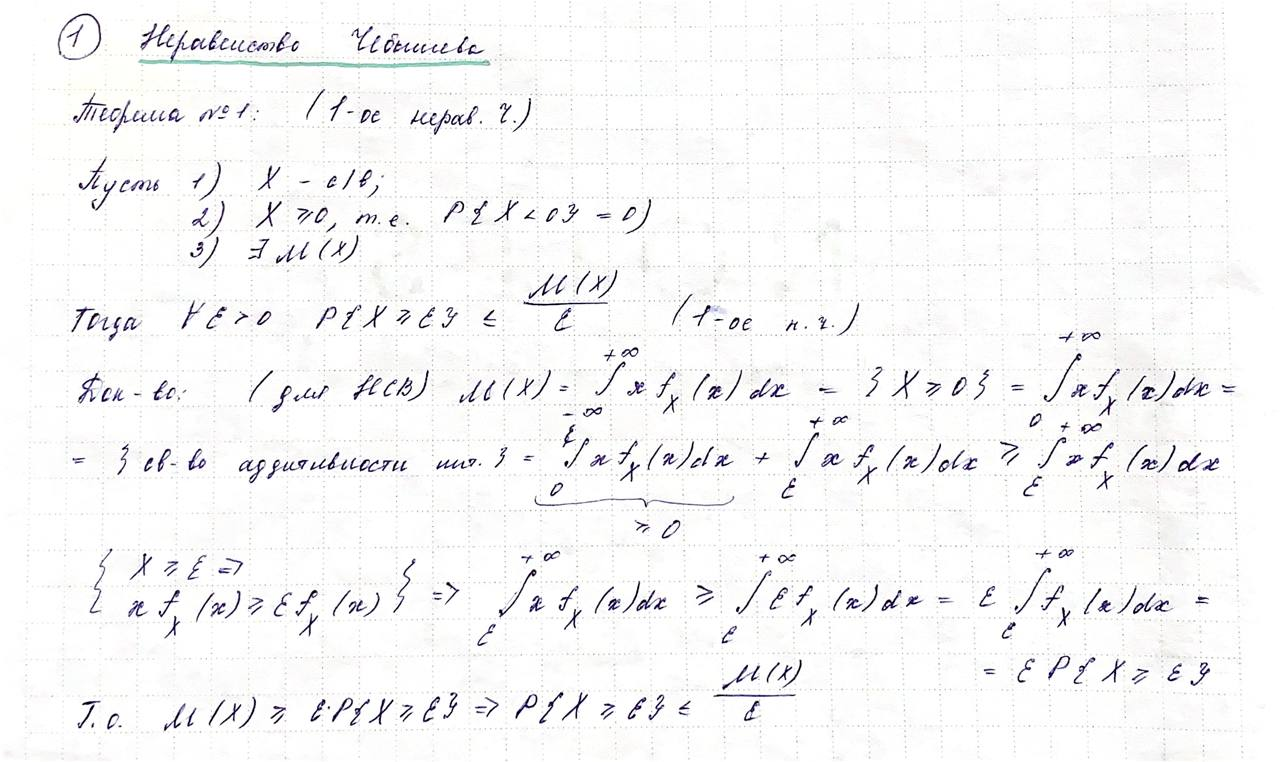
\includegraphics[scale=0.35]{pics/1.jpg}}
	\end{figure}
	\item \textbf{Сформулировать и доказать второе неравенство Чебышева.}
	\begin{figure}[!h]
		\center{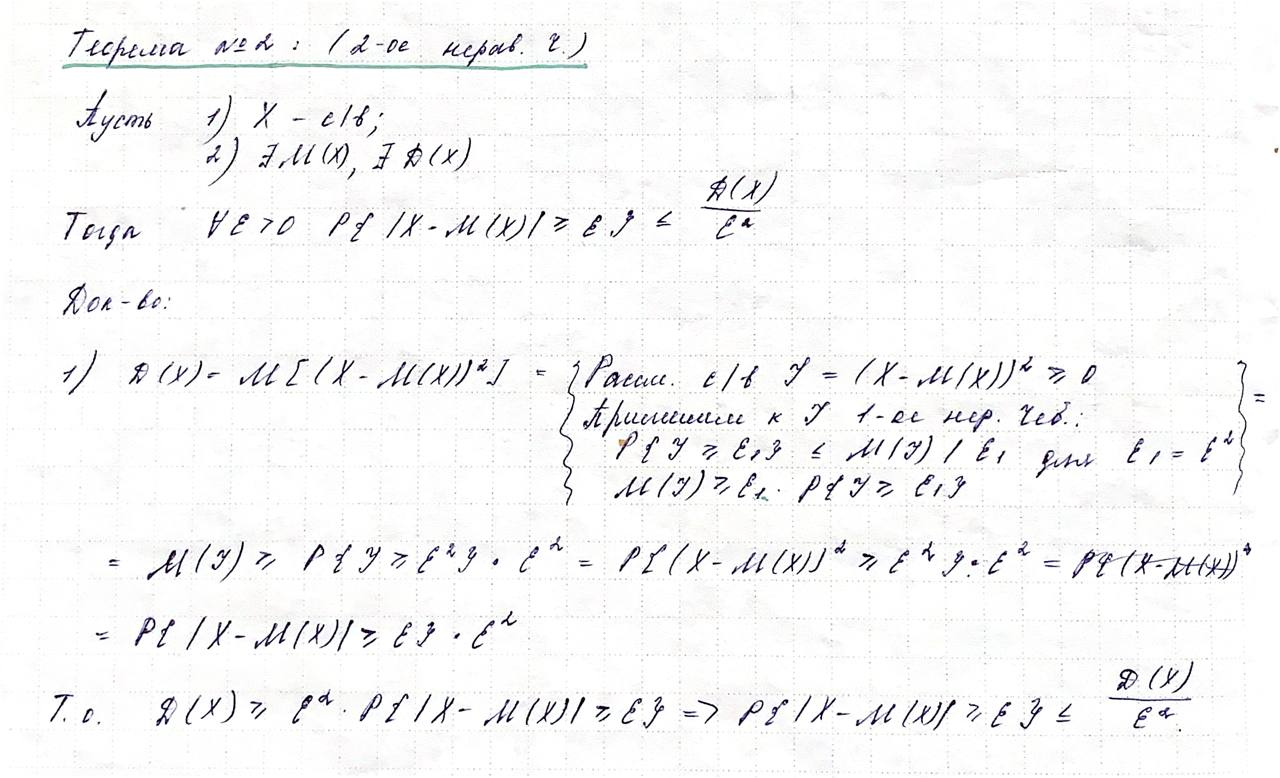
\includegraphics[scale=0.4]{pics/2.jpg}}
	\end{figure}
	\item \textbf{Для последовательности случайных величин сформулировать определения сходимости по вероятности и слабой сходимости. Сформулировать закон больших чисел.}
	\begin{figure}[!h]
		\center{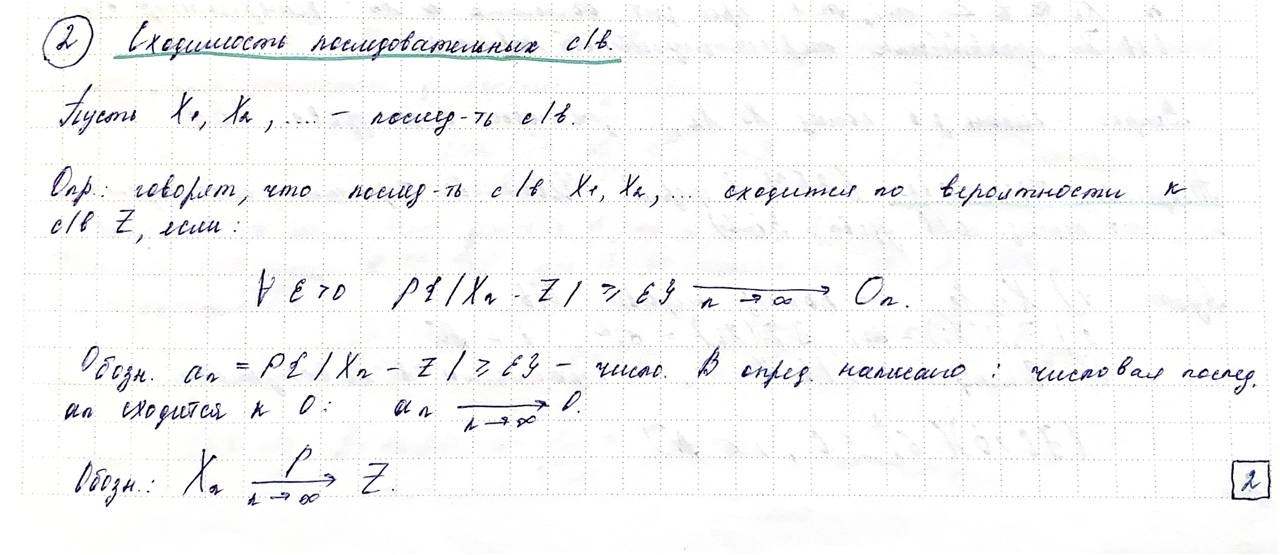
\includegraphics[scale=0.4]{pics/3_1.jpg}}
	\end{figure}
	\begin{figure}[!h]
		\center{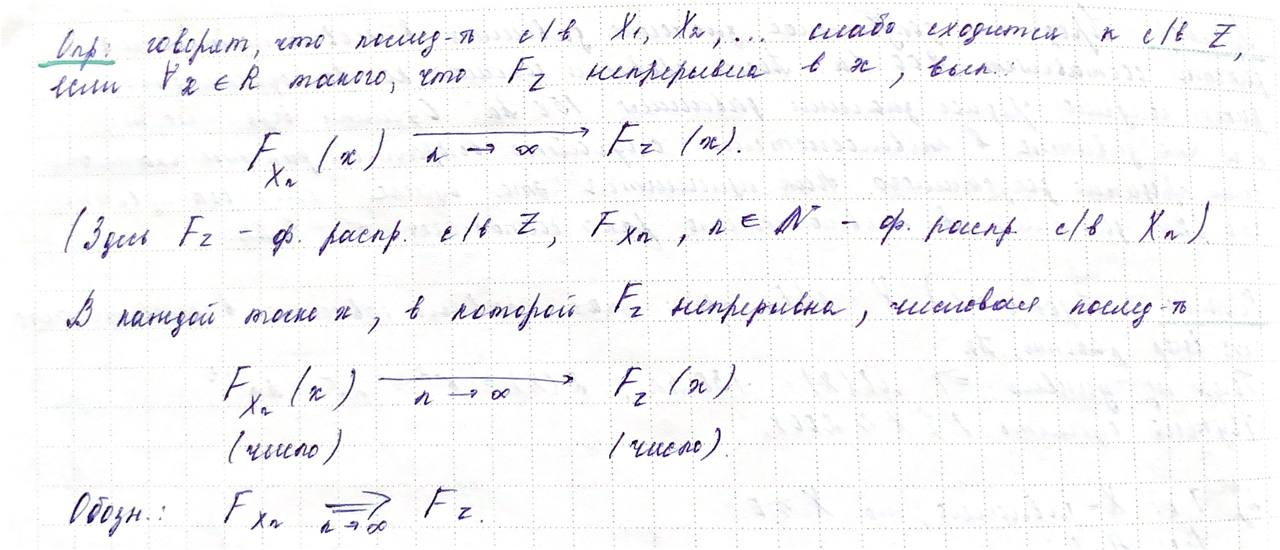
\includegraphics[scale=0.4]{pics/3_2.jpg}}
	\end{figure}
	\clearpage
	\item \textbf{Сформулировать закон больших чисел. Доказать закон больших чисел в форме Чебышева.}
	\begin{figure}[!h]
		\center{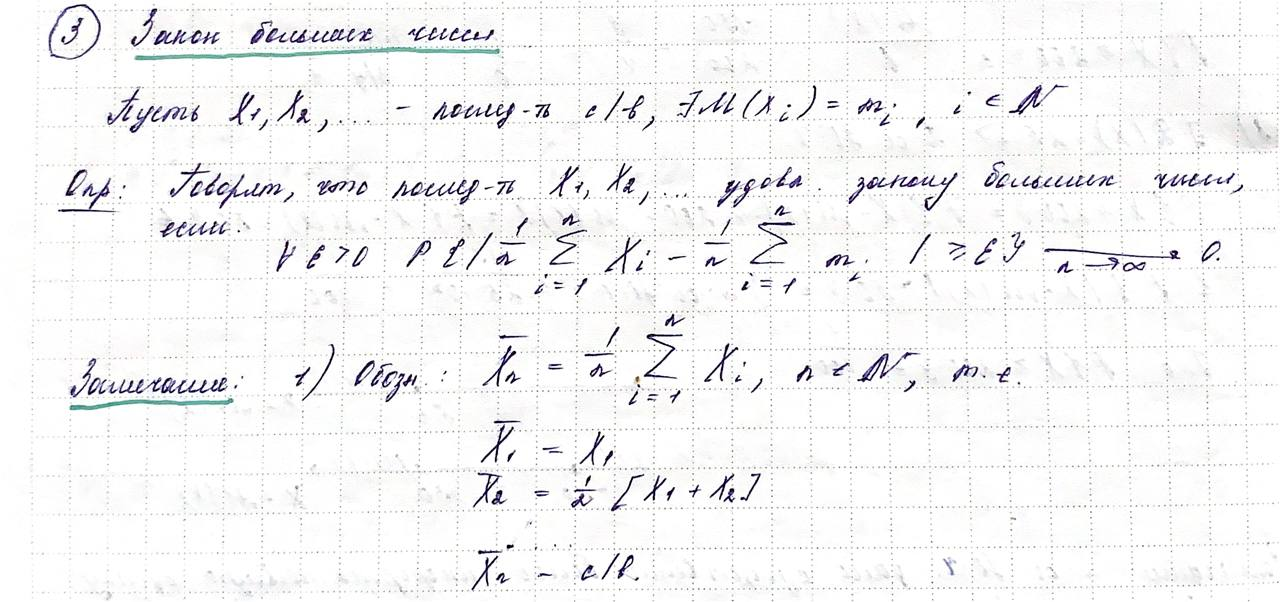
\includegraphics[scale=0.3]{pics/4_1.jpg}}
	\end{figure}
	\begin{figure}[!h]
		\center{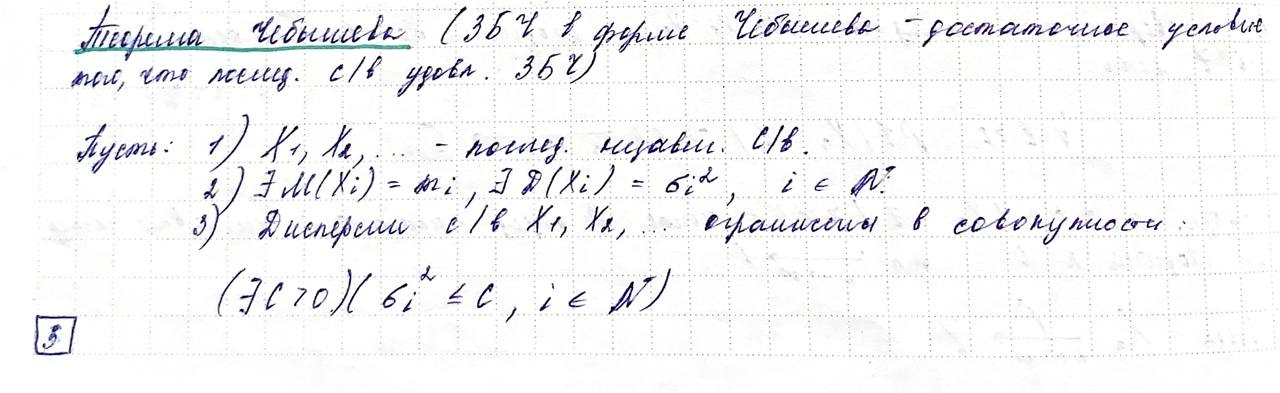
\includegraphics[scale=0.32]{pics/4_2.jpg}}
	\end{figure}
	\begin{figure}[!h]
		\center{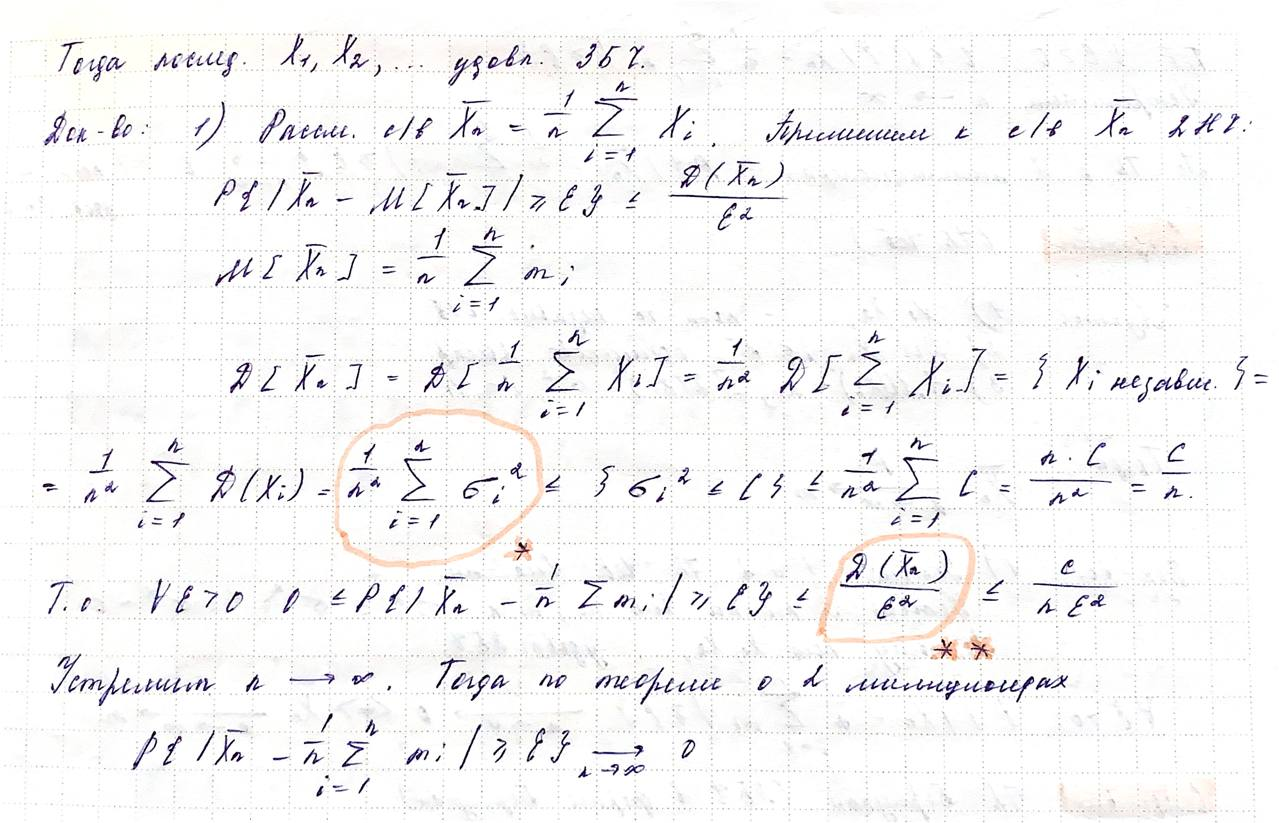
\includegraphics[scale=0.32]{pics/4_3.jpg}}
	\end{figure}
	\item \textbf{Сформулировать закон больших чисел в форме Чебышева. Доказать следствие этого закона
		для одинаково распределенных случайных величин и закон больших чисел в форме Бернулли.}
	
		Ответ на первый вопрос смотреть в ответах на вопрос 4.
		\begin{figure}[!h]
			\center{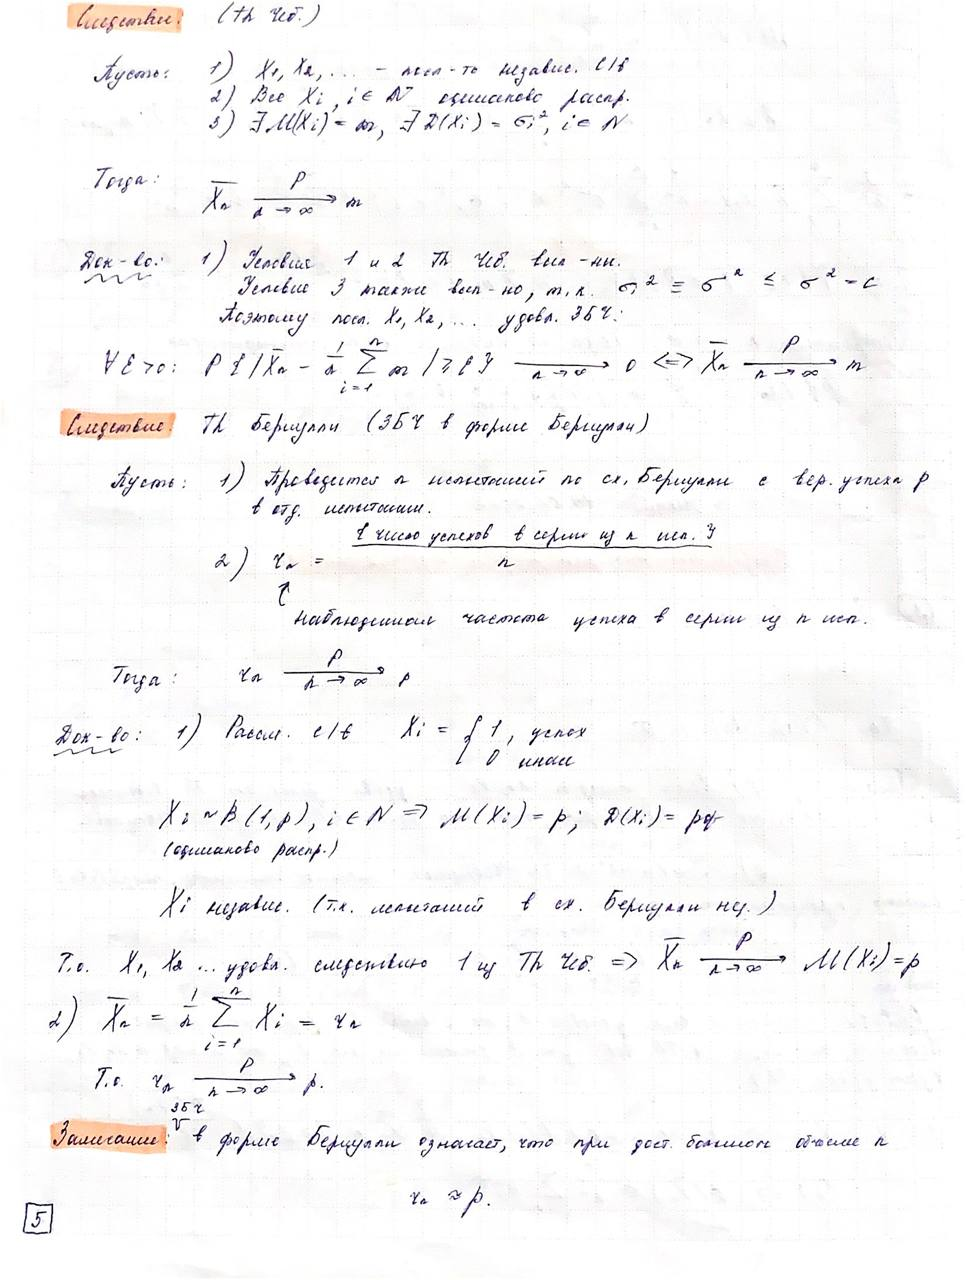
\includegraphics[scale=0.47]{pics/5.jpg}}
		\end{figure}
	\item \textbf{Сформулировать центральную предельную теорему. Доказать интегральную теорему
		Муавра-Лапласа.}
	\begin{figure}[!h]
		\center{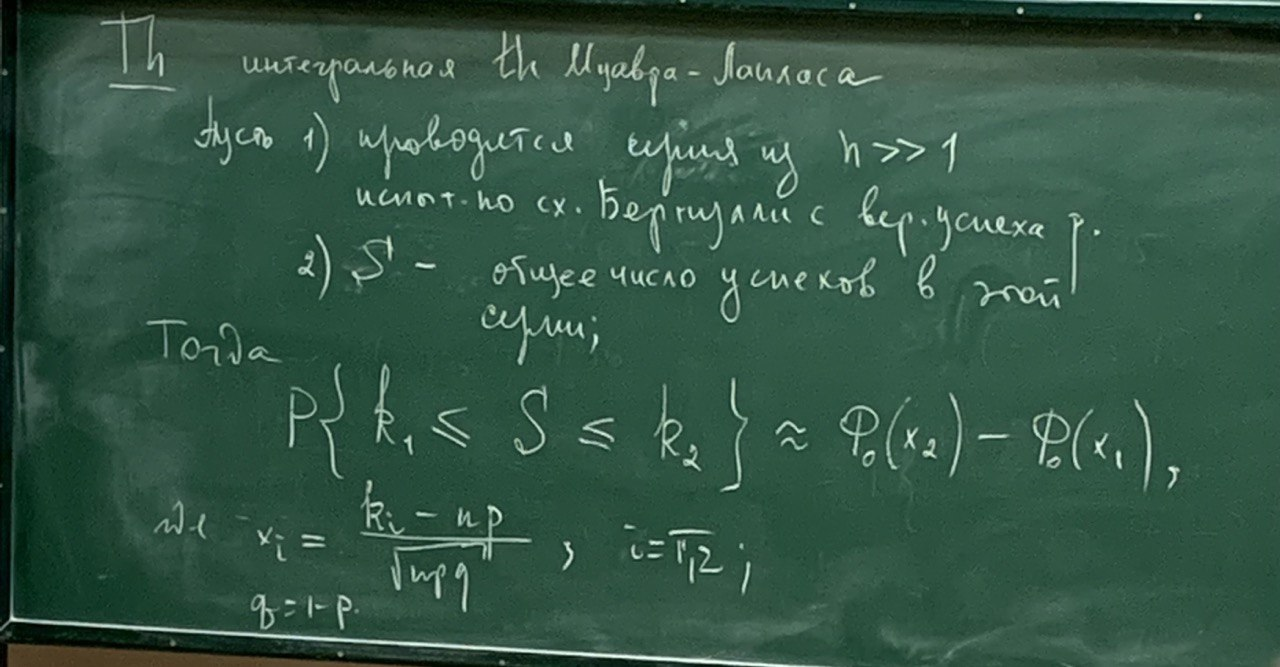
\includegraphics[scale=0.42]{pics/6_1.jpg}}
	\end{figure}
	\begin{figure}[!h]
		\center{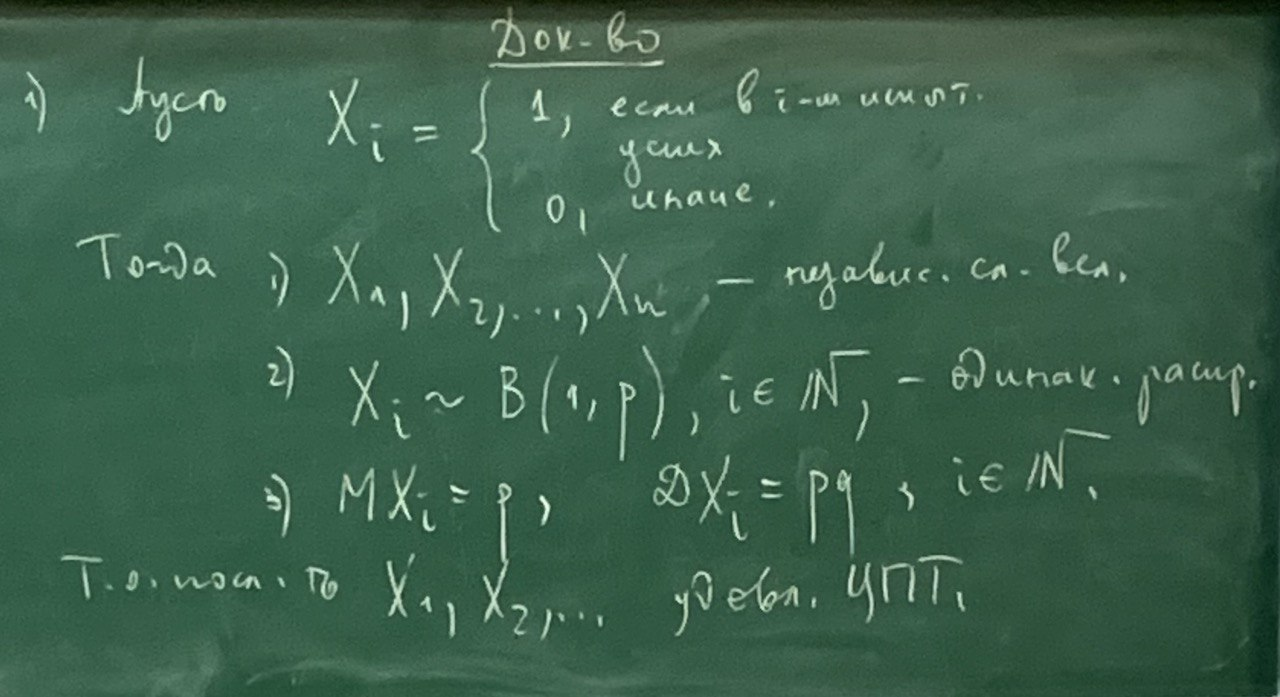
\includegraphics[scale=0.42]{pics/6_2.jpg}}
	\end{figure}
	\clearpage
	\begin{figure}[!h]
		\center{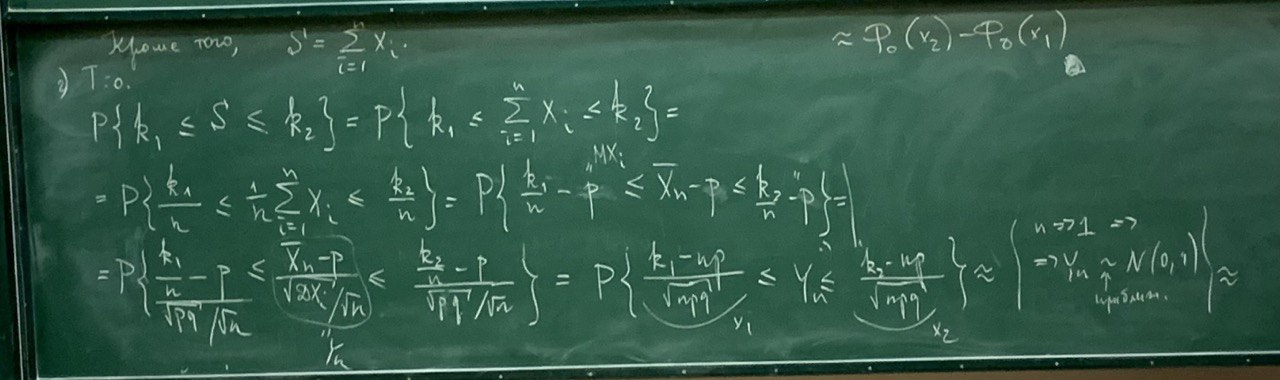
\includegraphics[scale=0.43]{pics/6_3.jpg}}
	\end{figure}
	\item \textbf{Сформулировать определение случайной выборки и выборки, вариационного ряда. Записать
		и обосновать выражения для функций распределения случайной выборки и крайних членов
		вариационного ряда.}
	\begin{figure}[!h]
		\center{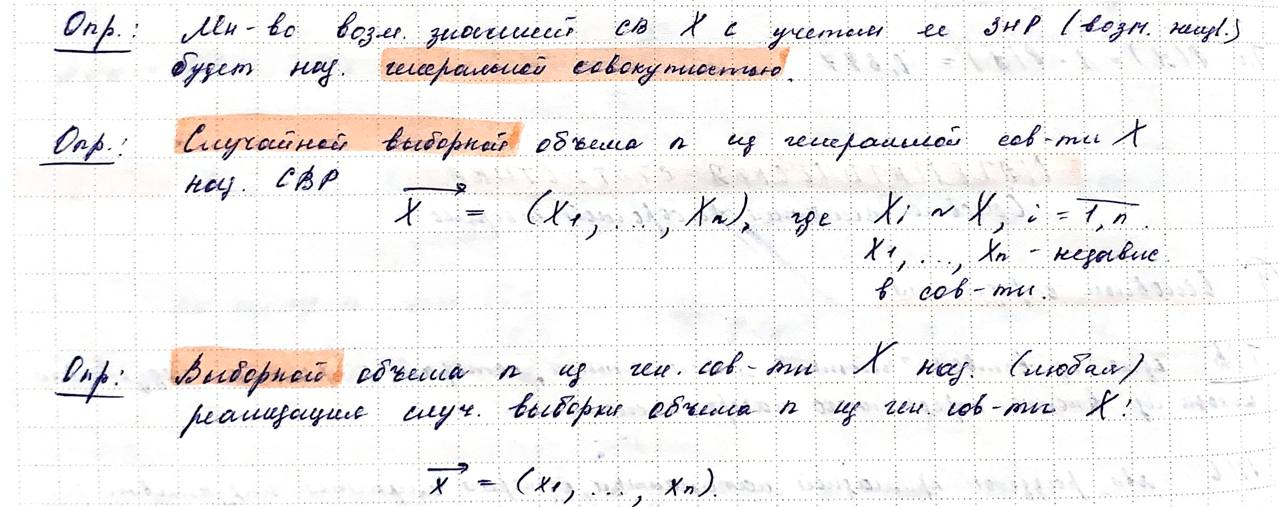
\includegraphics[scale=0.32]{pics/7_1.jpg}}
	\end{figure}
	\begin{figure}[!h]
		\center{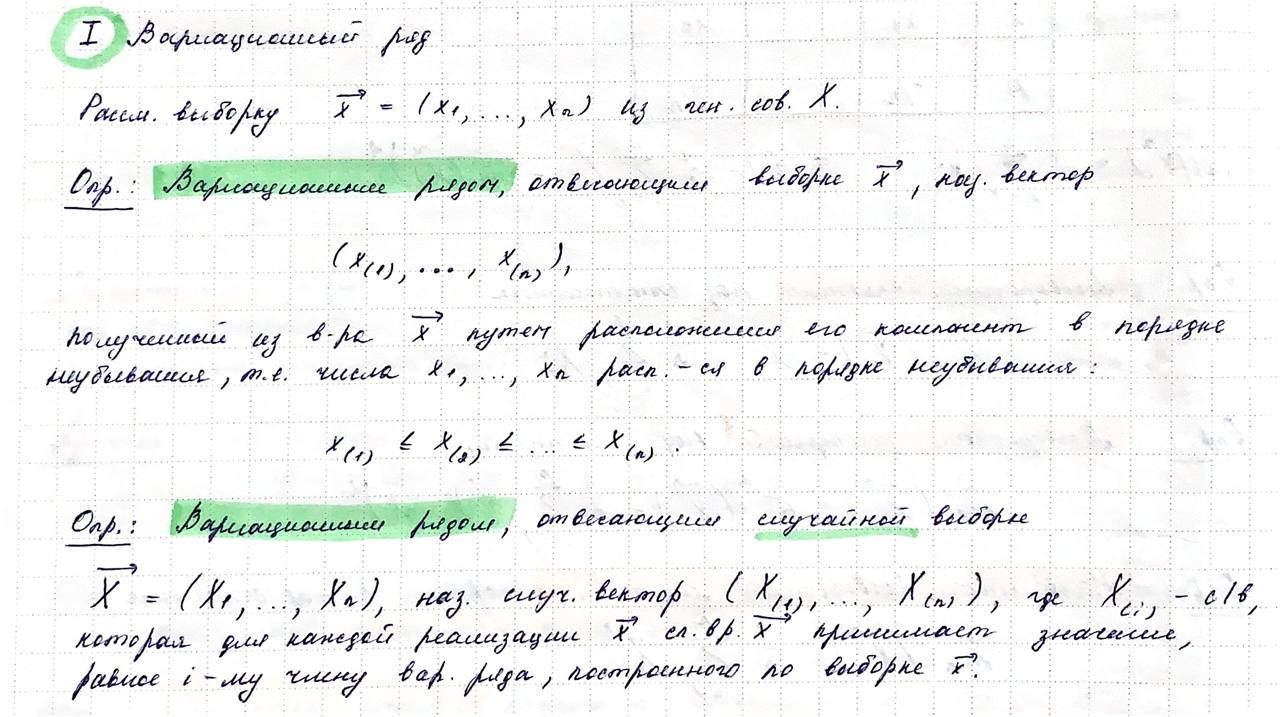
\includegraphics[scale=0.33]{pics/7_2.jpg}}
	\end{figure}
	\begin{figure}[!h]
		\center{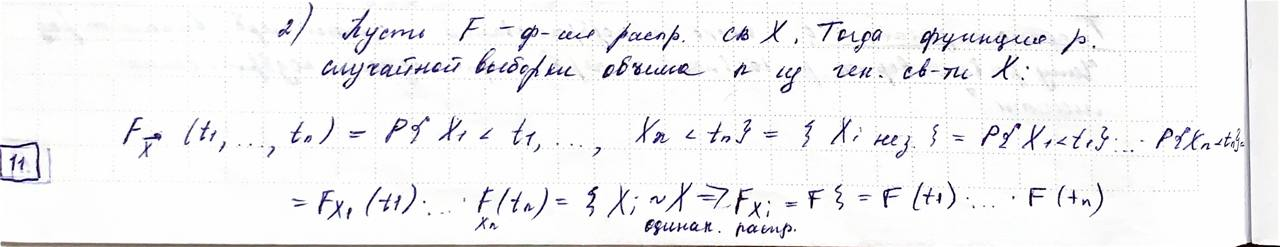
\includegraphics[scale=0.4]{pics/7_3.jpg}}
	\end{figure}
	\textcolor{red}{Про крайние значения я ничего в лекциях не нашла, мб имеется в виду из вариационного ряда $x_{(i)}$}
	
	\item \textbf{Сформулировать определение начальных и центральных выборочных моментов порядка k,
		выборочного среднего и выборочной дисперсии. Являются ли эти статистики несмещенными
		оценками своих теоретических аналогов?}
	
	\begin{figure}[!h]
		\center{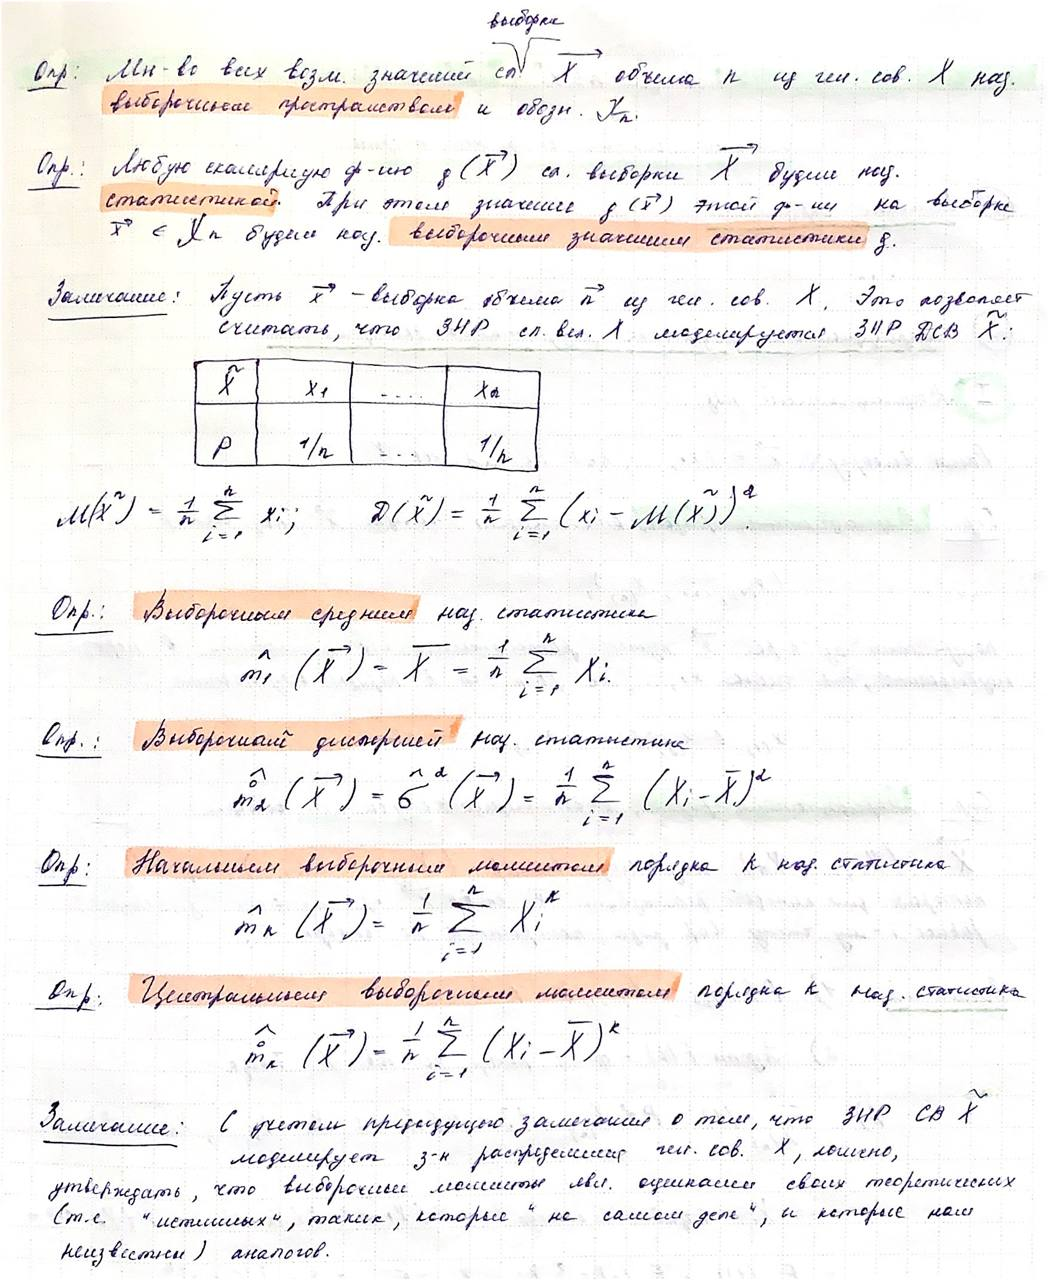
\includegraphics[scale=0.35]{pics/8_1.jpg}}
	\end{figure}

	\textcolor{red}{Про несмещенность пока не нашла}
	
	\item \textbf{Сформулировать определения эмпирической функции распределения и выборочной функции
		распределения. Сформулировать и доказать теорему о сходимости выборочной функции распределения.}
	
	\begin{figure}[!h]
		\center{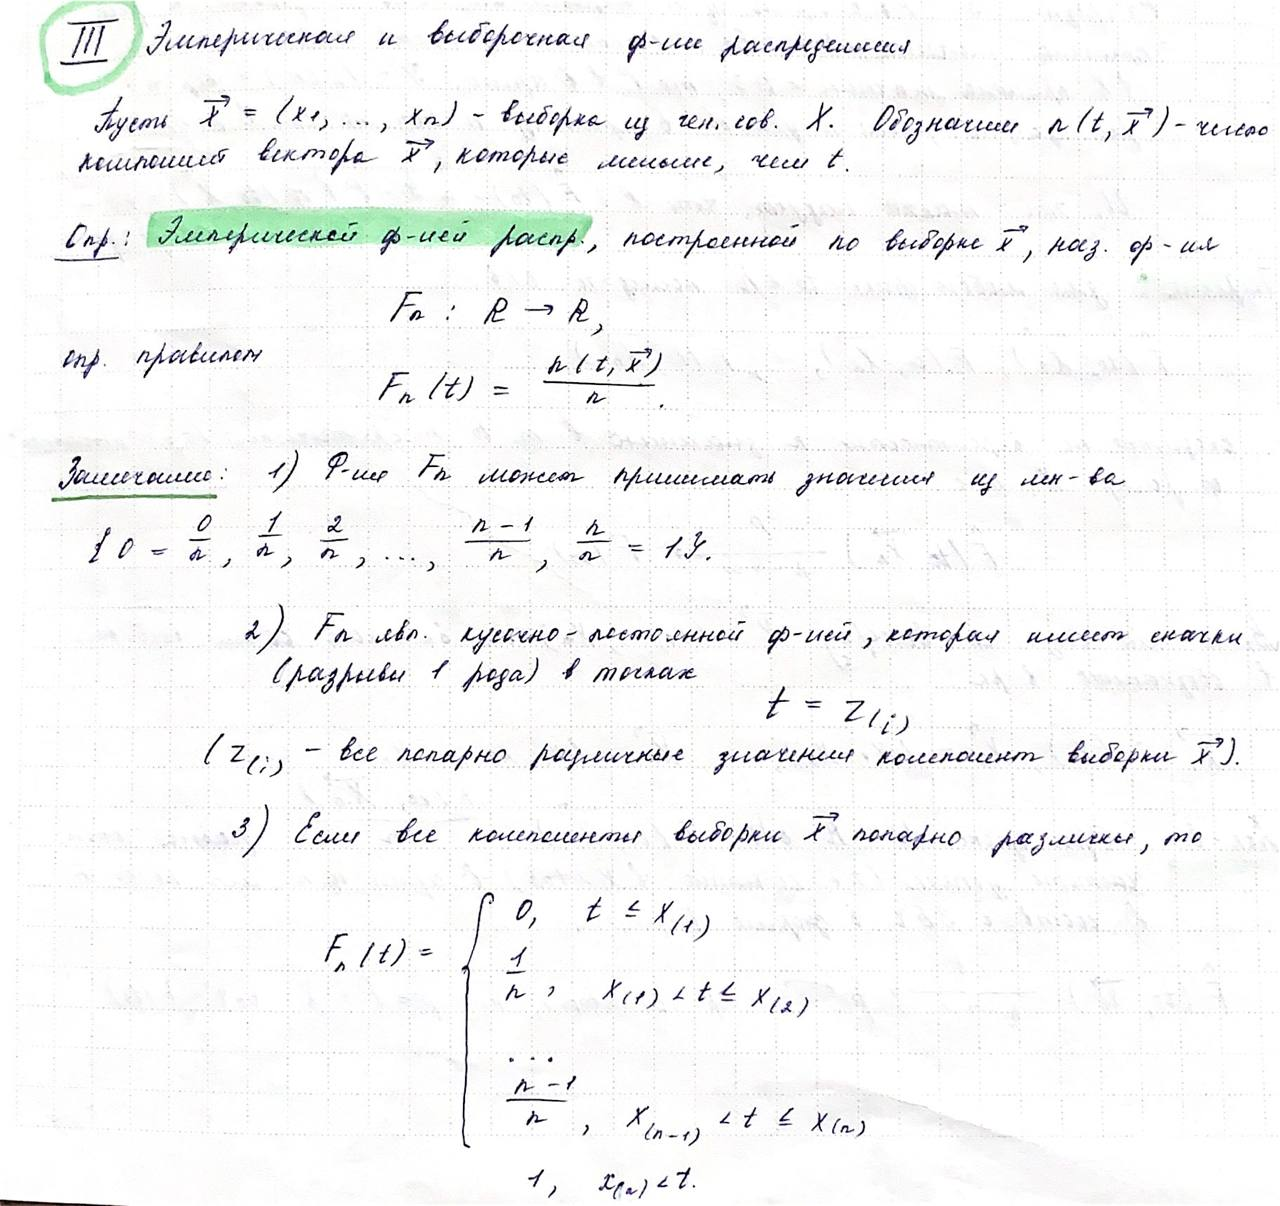
\includegraphics[scale=0.27]{pics/9_1.jpg}}
	\end{figure}
	\begin{figure}[!h]
		\center{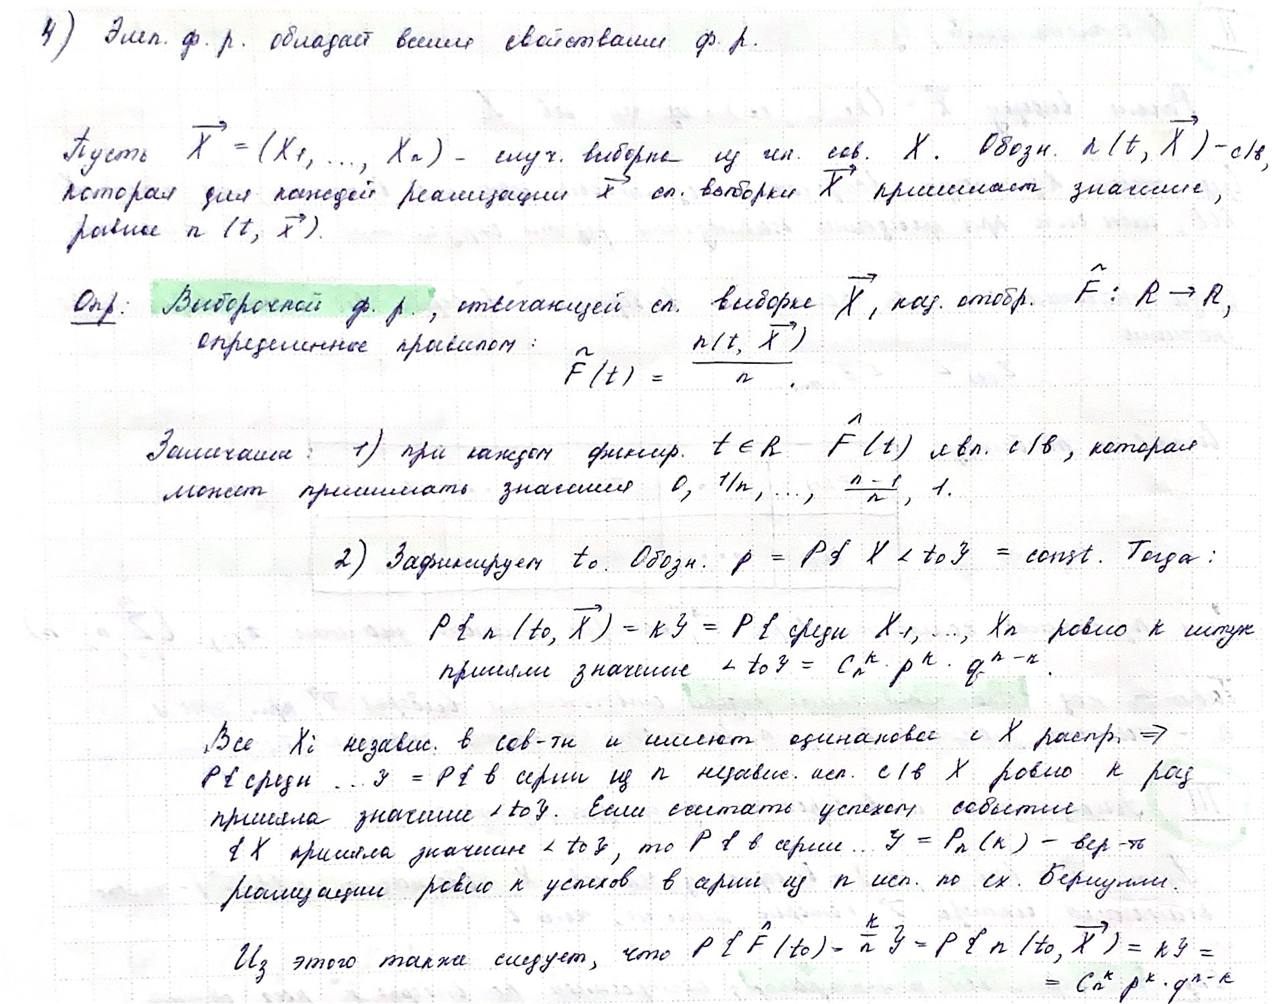
\includegraphics[scale=0.27]{pics/9_2.jpg}}
	\end{figure}
	\begin{figure}[!h]
		\center{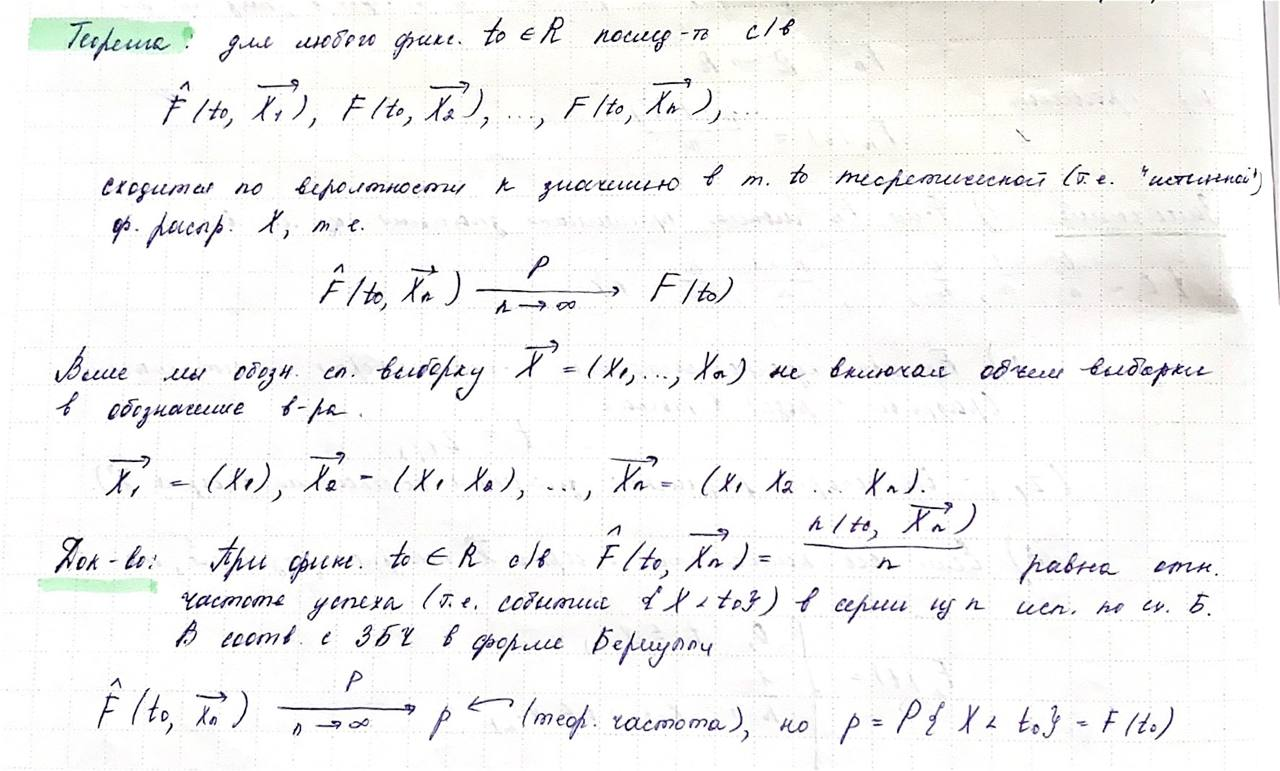
\includegraphics[scale=0.35]{pics/9_3.jpg}}
	\end{figure}

	\item \textbf{Понятия интервального статистического ряда, эмпирической плотности, гистограммы, полигона частот.}
	
	\begin{figure}[!h]
		\center{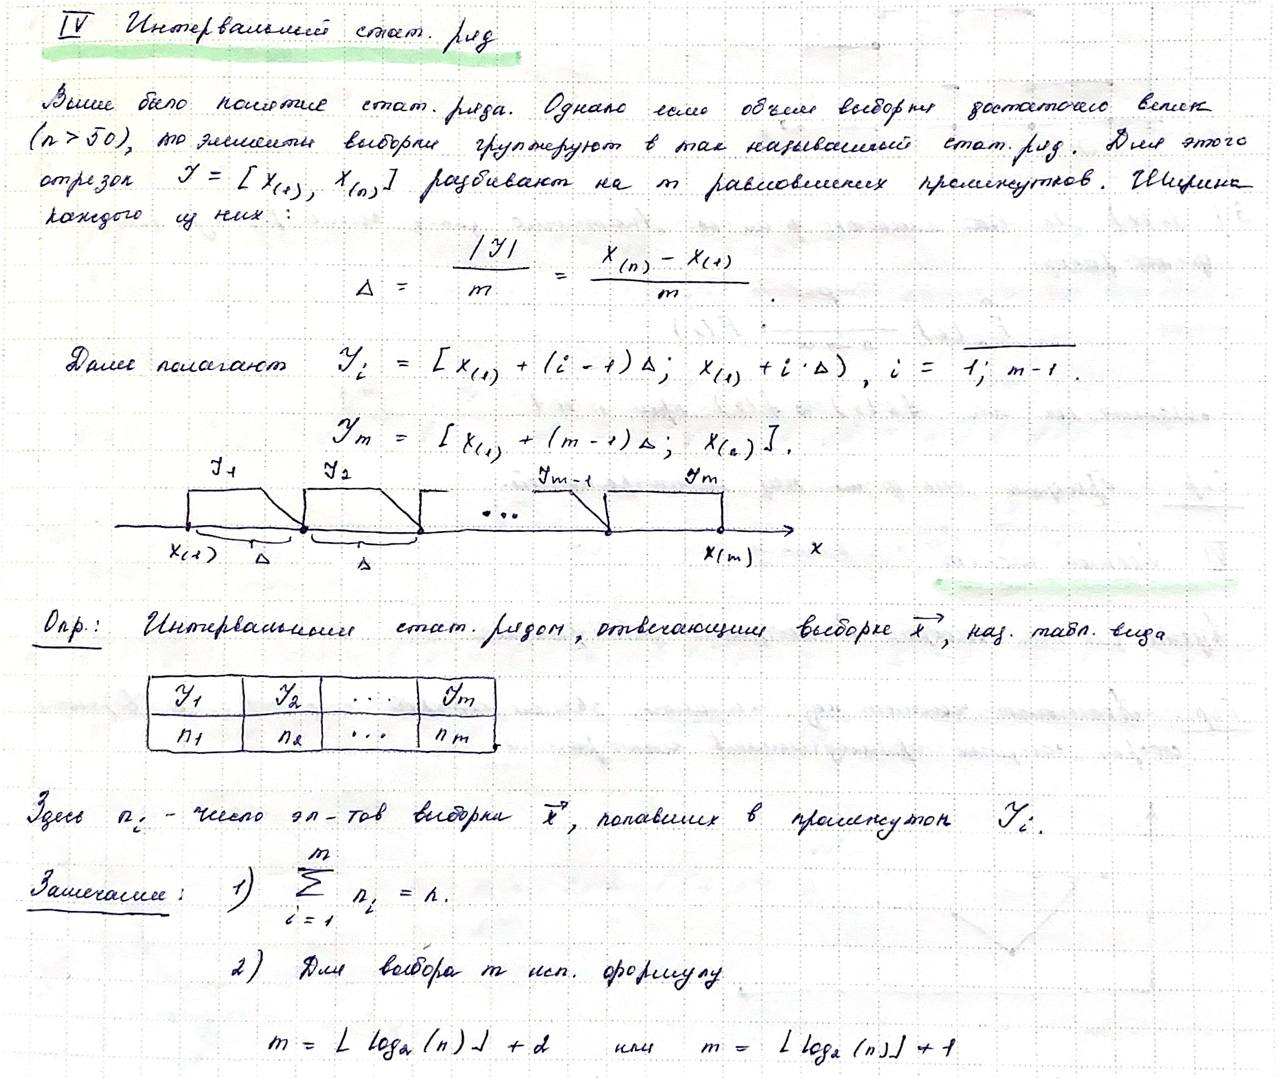
\includegraphics[scale=0.32]{pics/10_1.jpg}}
	\end{figure}
	\begin{figure}[!h]
		\center{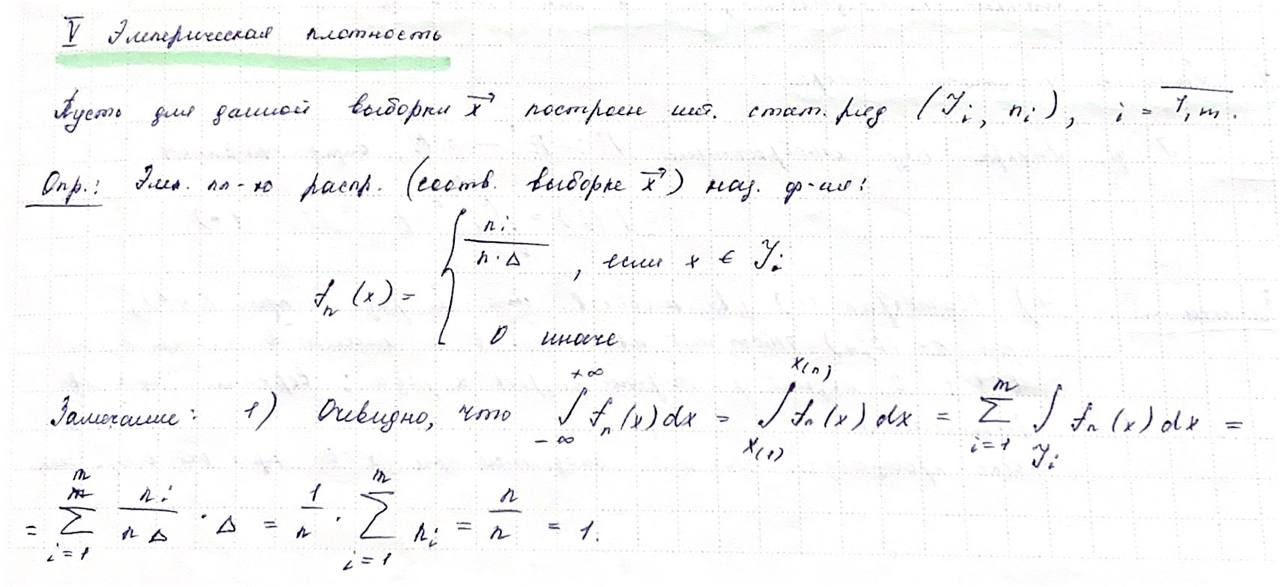
\includegraphics[scale=0.33]{pics/10_2.jpg}}
	\end{figure}
	\begin{figure}[!h]
		\center{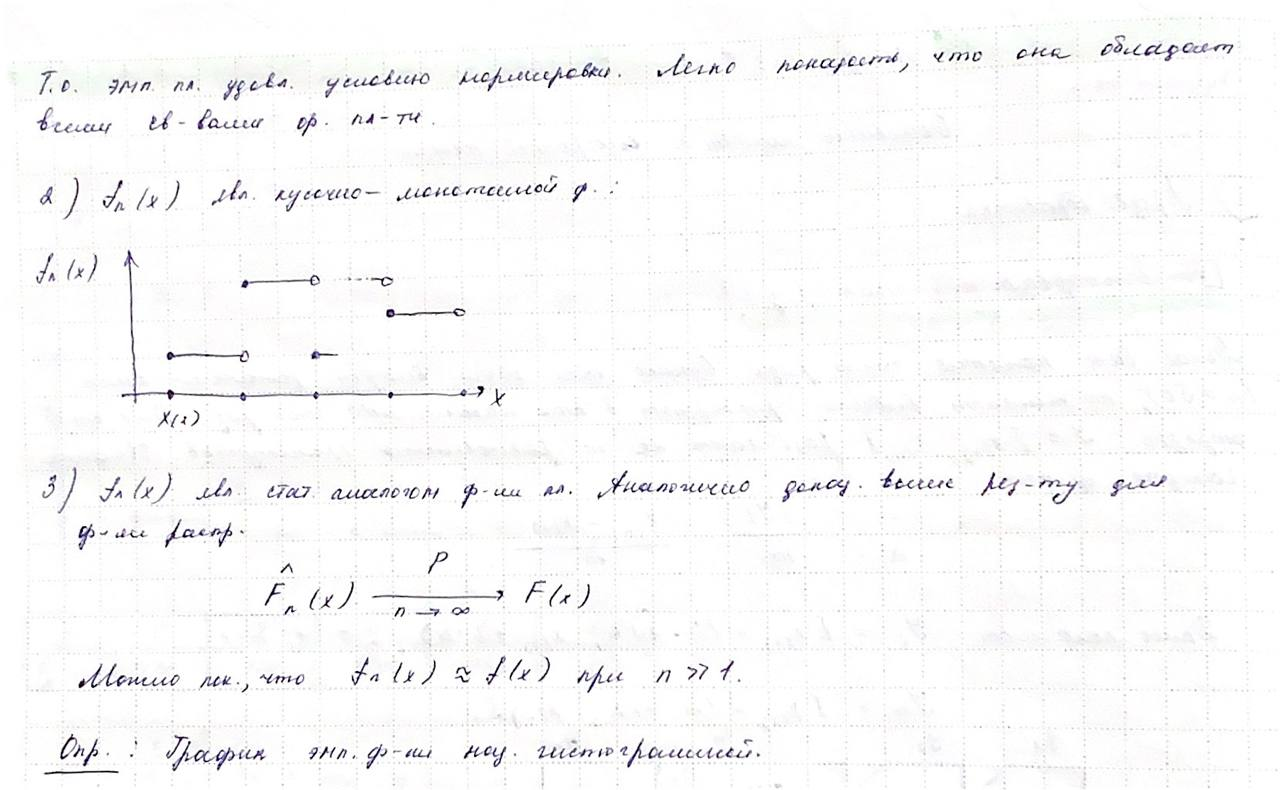
\includegraphics[scale=0.33]{pics/10_3.jpg}}
	\end{figure}
	\begin{figure}[!h]
		\center{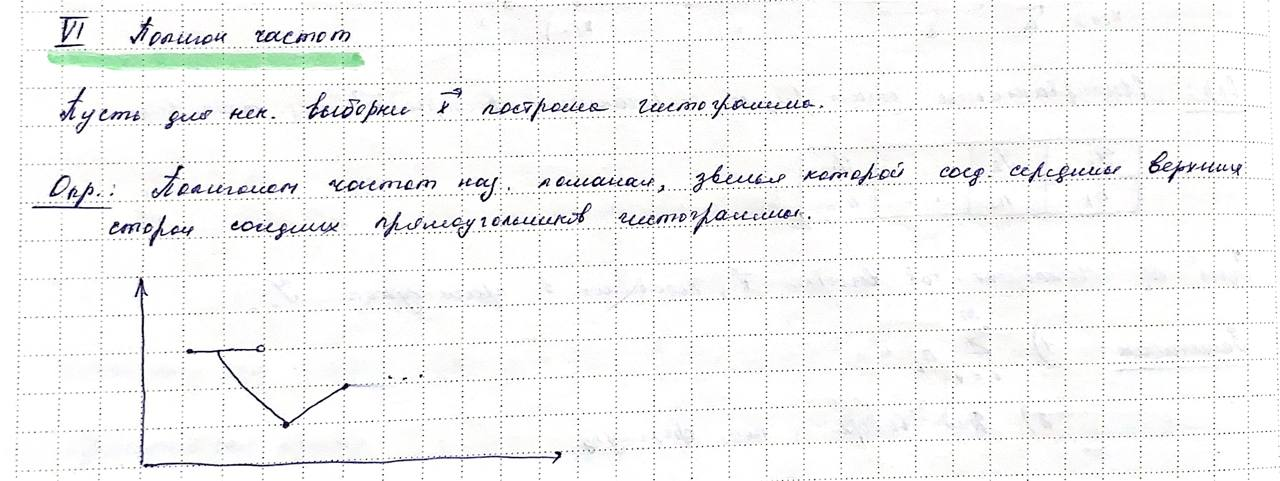
\includegraphics[scale=0.32]{pics/10_4.jpg}}
	\end{figure}
	
	\item \textbf{Постановка задачи идентификации неизвестных параметров закона распределения случайной величины. Определение точечной оценки. Определение несмещенной точечной оценки. Показать, что выборочная дисперсия является смещенной оценкой дисперсии. Записать формулу
		для исправленной выборочной дисперсии.}
	
	\textcolor{red}{Не уверена, что задача ид-ции именно такая, но похоже на правду.}
	
	\begin{figure}[!h]
		\center{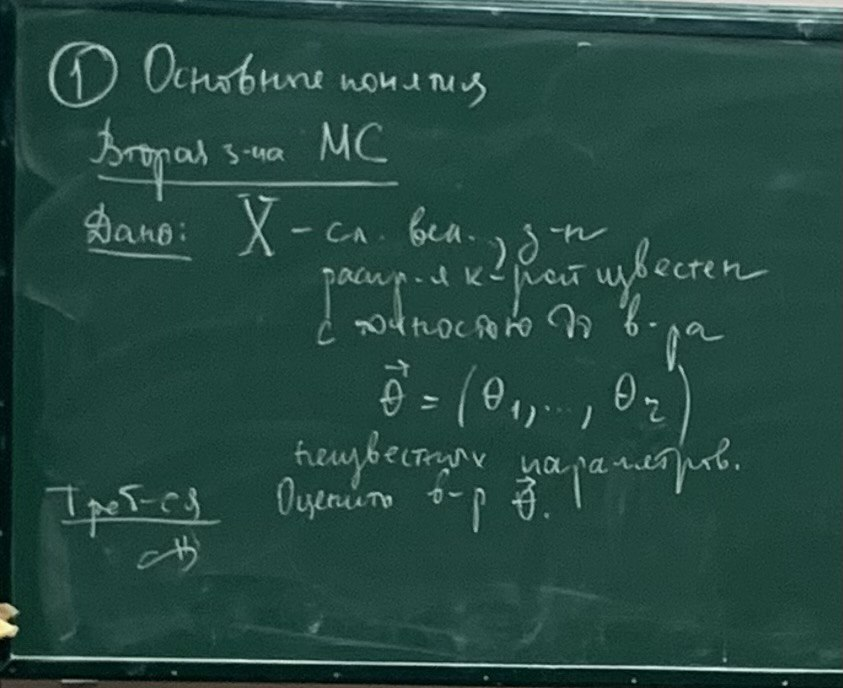
\includegraphics[scale=0.44]{pics/11_1.jpg}}
	\end{figure}
	\begin{figure}[!h]
		\center{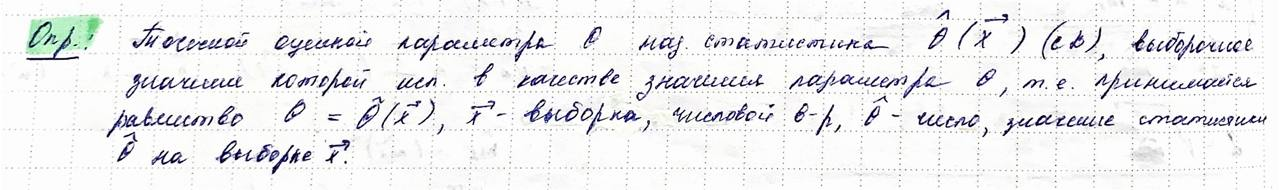
\includegraphics[scale=0.42]{pics/11_2.jpg}}
	\end{figure}
	\begin{figure}[!h]
		\center{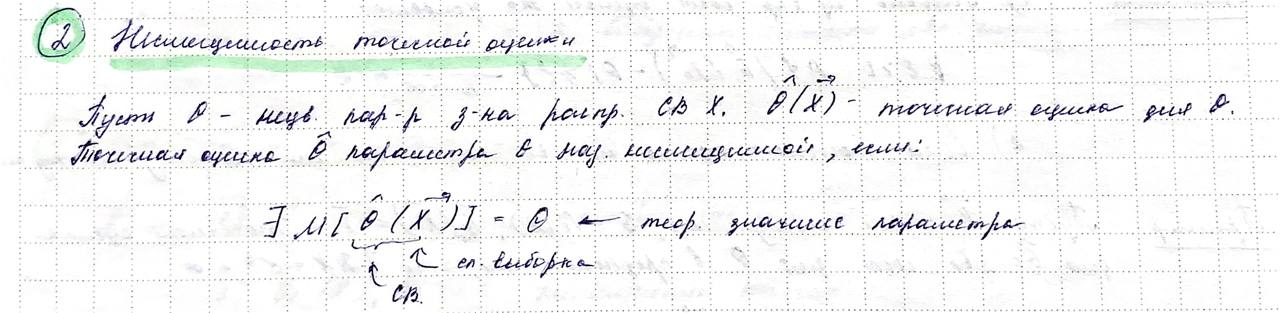
\includegraphics[scale=0.42]{pics/11_3.jpg}}
	\end{figure}
	\begin{figure}[!h]
		\center{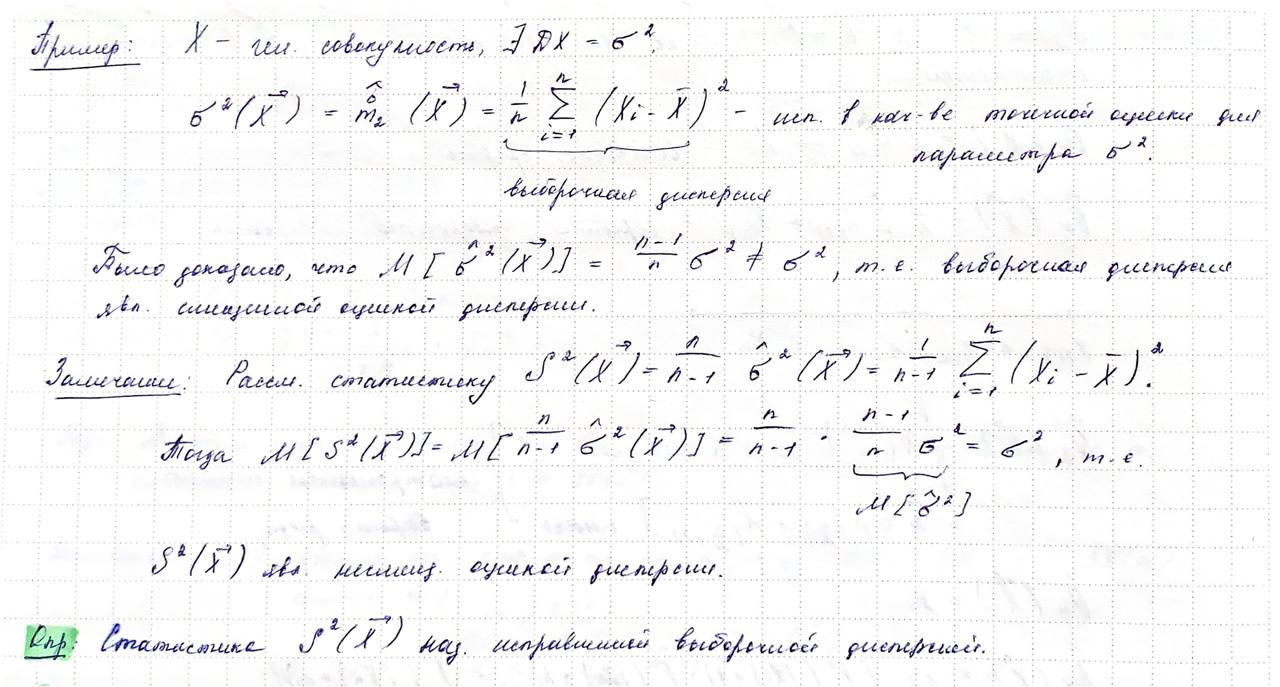
\includegraphics[scale=0.4]{pics/11_4.jpg}}
	\end{figure}
	
	\item \textbf{Постановка задачи идентификации неизвестных параметров закона распределения случайной величины. Определение точечной оценки. Определение состоятельной оценки. Привести
		примеры состоятельной и несостоятельной оценок (с обоснованием).}
	
	Ответ на первый и второй вопрос смотреть в ответах на вопрос 11.
	
	\begin{figure}[!h]
		\center{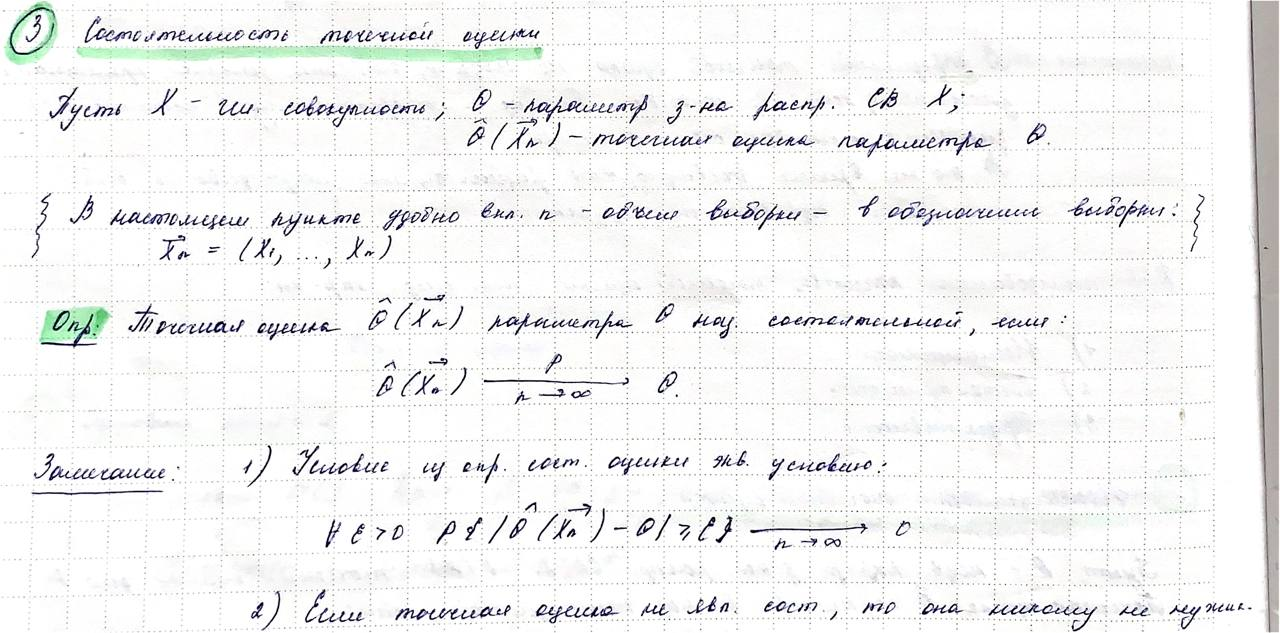
\includegraphics[scale=0.43]{pics/12_1.jpg}}
	\end{figure}
	\begin{figure}[!h]
		\center{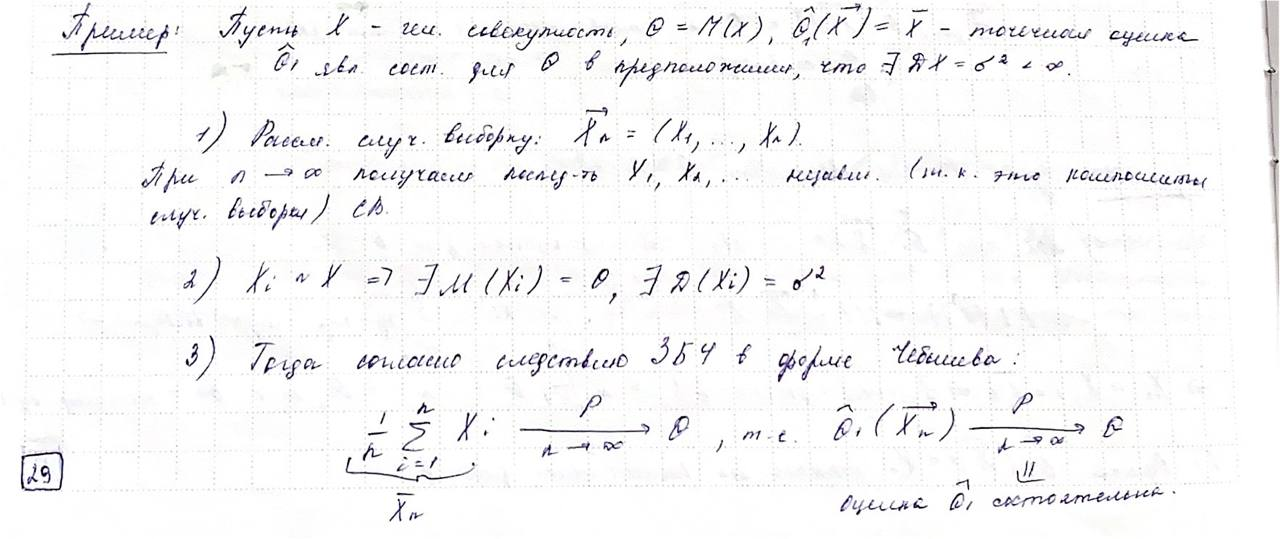
\includegraphics[scale=0.36]{pics/12_2.jpg}}
	\end{figure}
	\begin{figure}[!h]
		\center{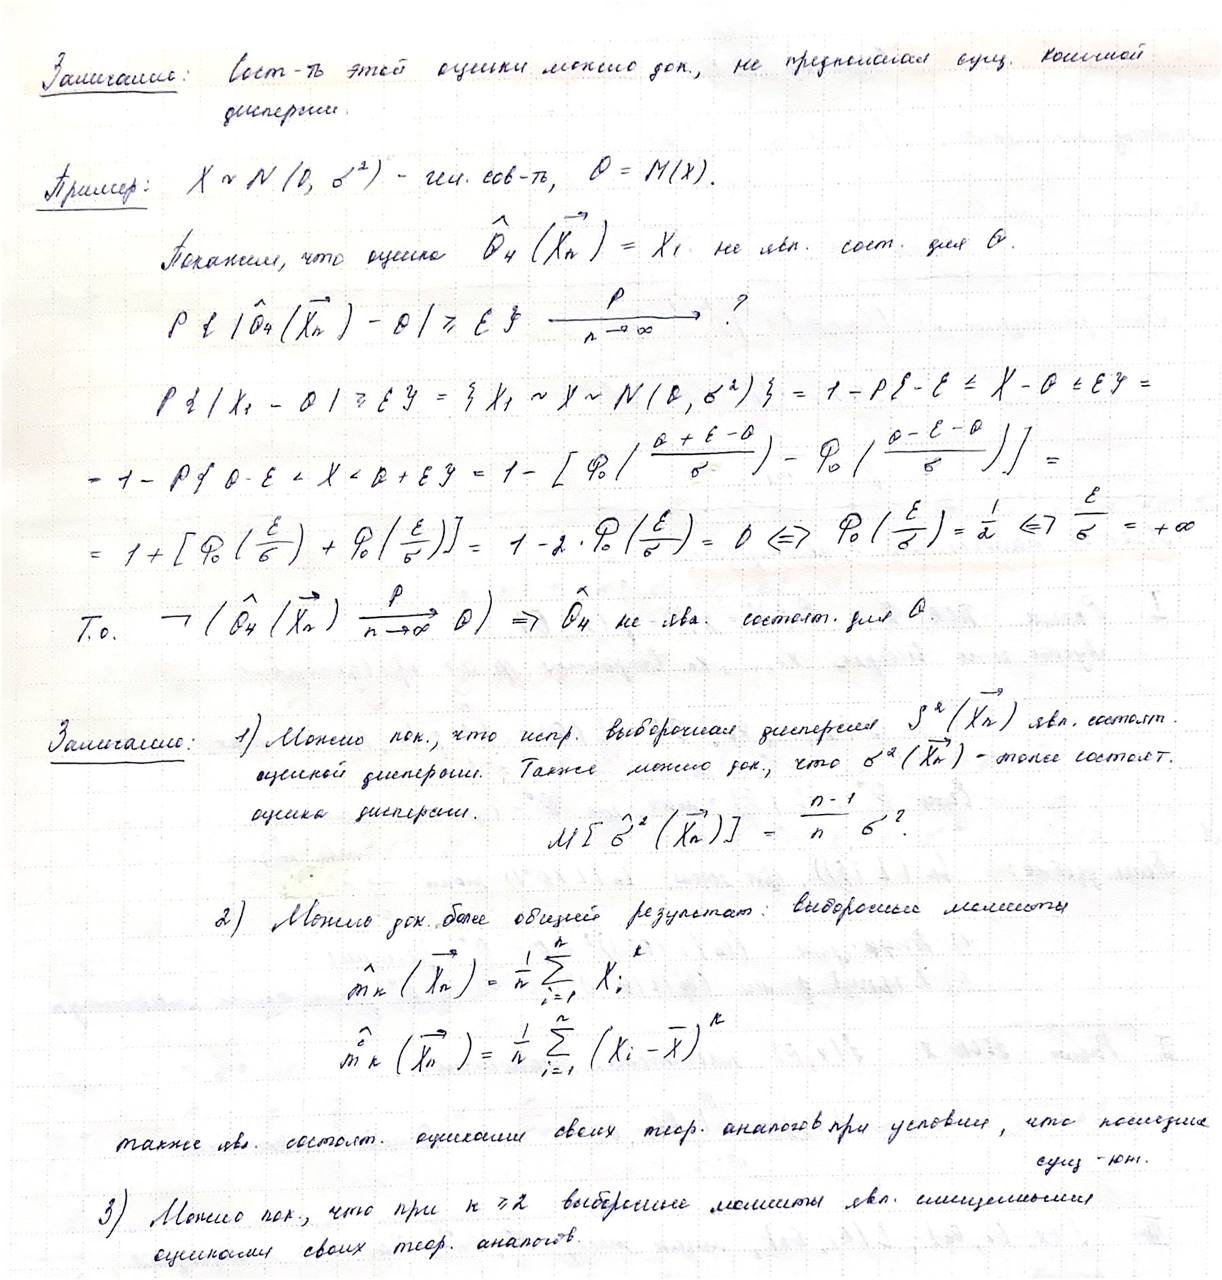
\includegraphics[scale=0.35]{pics/12_3.jpg}}
	\end{figure}
	
	\item \textbf{Постановка задачи идентификации неизвестных параметров закона распределения случайной величины. Определение точечной оценки. Определение эффективной оценки. Показать,
		что выборочное среднее является эффективной оценкой математического ожидания в классе
		линейных оценок.}
	
	Ответ на первый и второй вопрос смотреть в ответах на вопрос 11.
	
	\begin{figure}[!h]
		\center{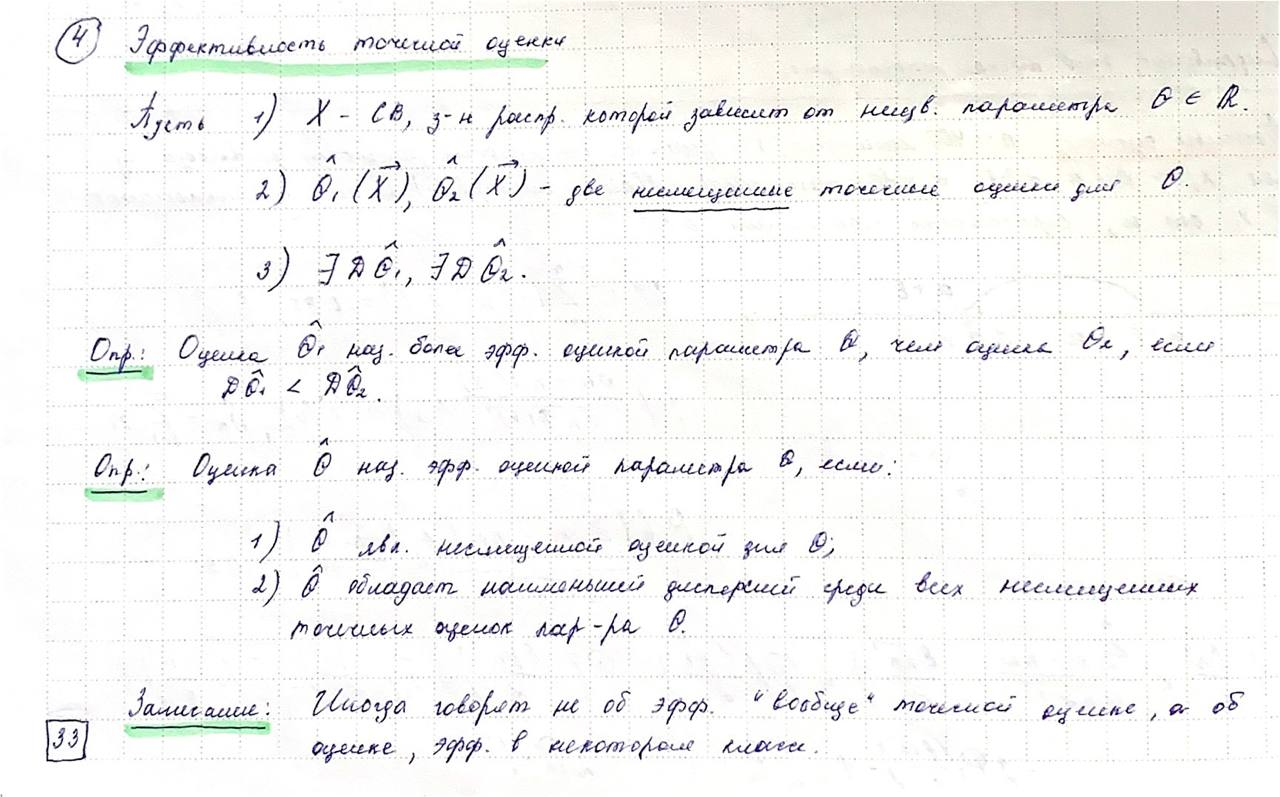
\includegraphics[scale=0.4]{pics/13_1.jpg}}
	\end{figure}
	\clearpage
	\begin{figure}[!h]
		\center{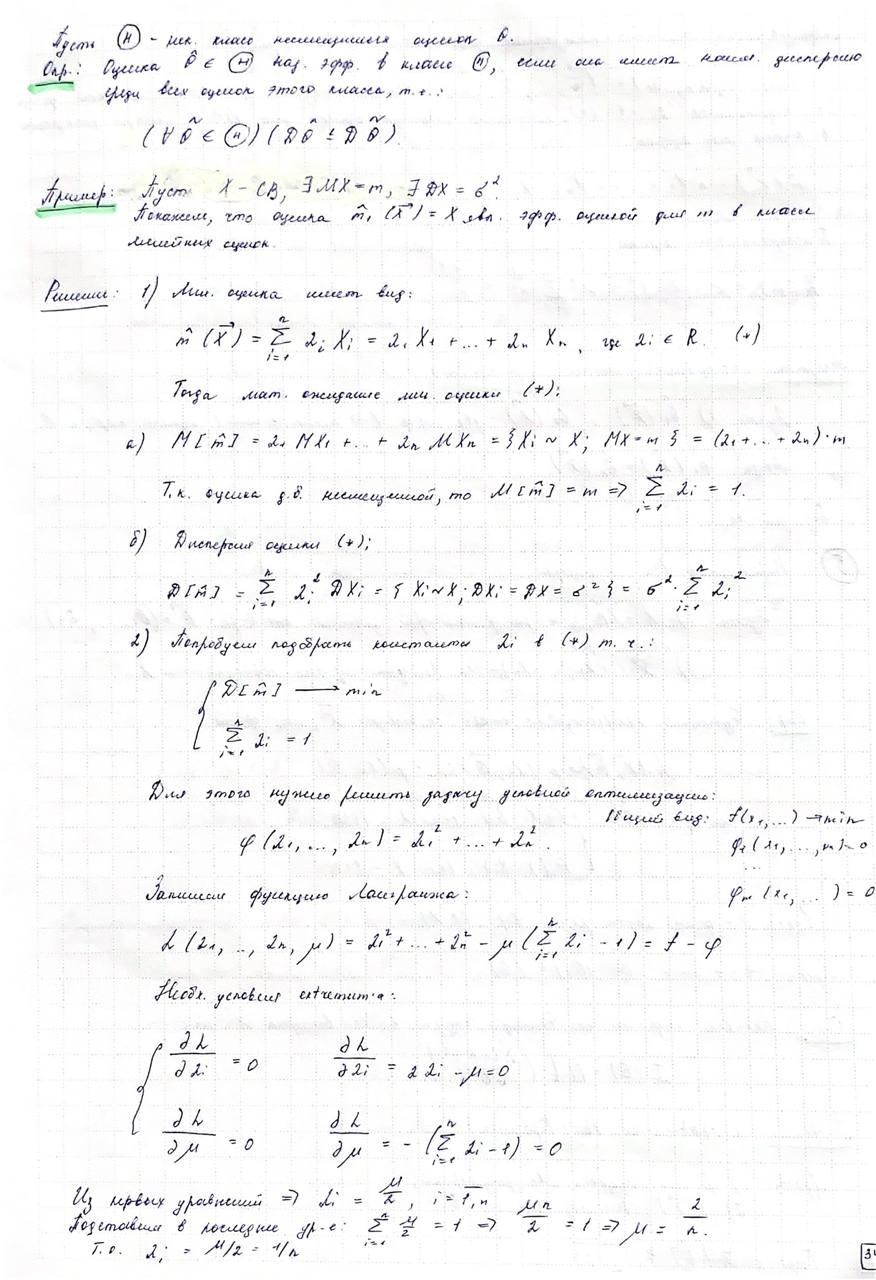
\includegraphics[scale=0.51]{pics/13_2.jpg}}
	\end{figure}
	\begin{figure}[!h]
		\center{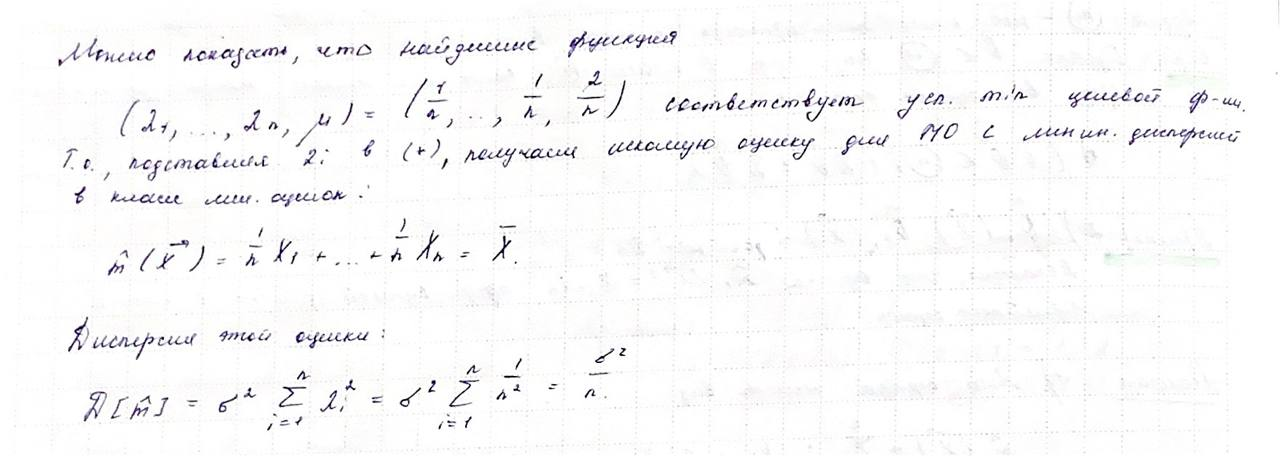
\includegraphics[scale=0.4]{pics/13_3.jpg}}
	\end{figure}
	
	\item \textbf{Постановка задачи идентификации неизвестных параметров закона распределения случайной величины. Определение точечной оценки. Определение эффективной оценки. Сформулировать теорему о единственности эффективной оценки.}
	
	Ответ на первый и второй вопрос смотреть в ответах на вопрос 11.
	
	Ответ на третий вопрос в ответах на вопрос 13.
	
	\begin{figure}[!h]
		\center{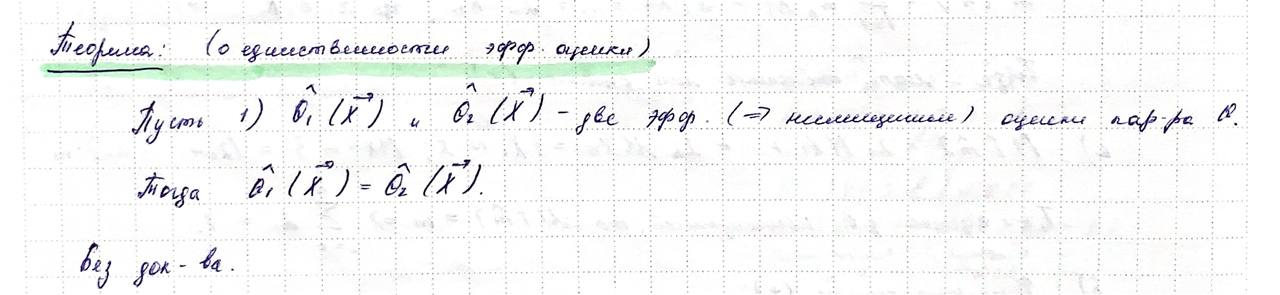
\includegraphics[scale=0.4]{pics/14_1.jpg}}
	\end{figure}
	
	\item \textbf{Постановка задачи идентификации неизвестных параметров закона распределения случайной величины. Определение точечной оценки. Определение эффективной оценки. Определение
		количества информации по Фишеру. Сформулировать теорему о неравенстве Рао-Крамера.}
	
	Ответ на первый и второй вопрос смотреть в ответах на вопрос 11.
	
	Ответ на третий вопрос в ответах на вопрос 13.
	
	\clearpage
	
	\begin{figure}[!h]
		\center{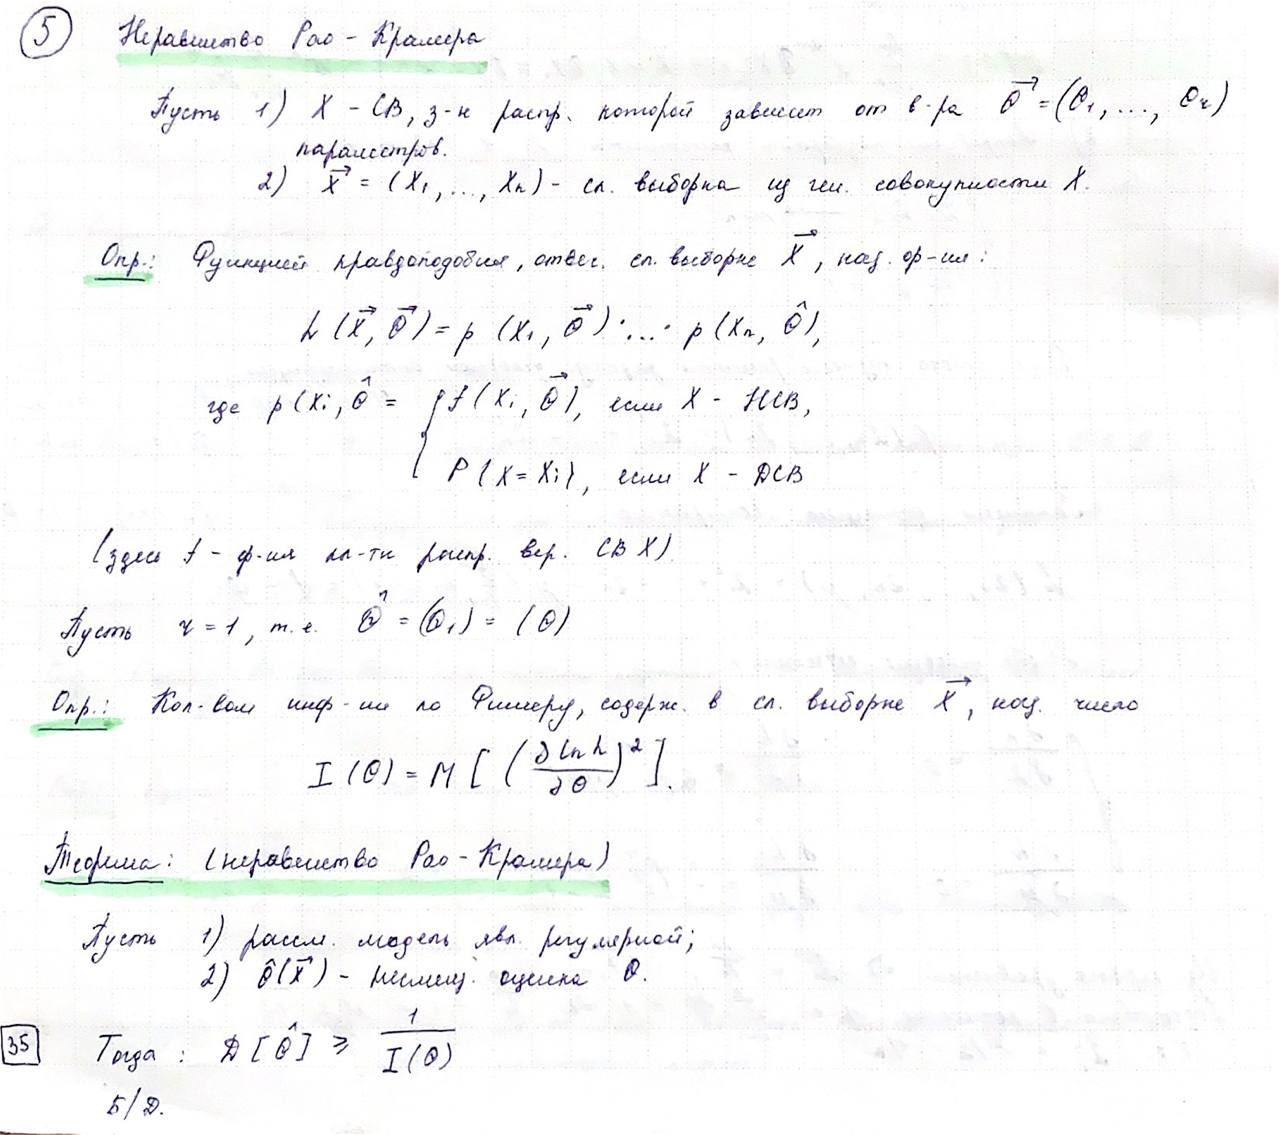
\includegraphics[scale=0.43]{pics/15_1.jpg}}
	\end{figure}
	
	\item \textbf{Постановка задачи идентификации неизвестных параметров закона распределения случайной величины. Определение точечной оценки. Определение эффективной оценки. Показать, что
		выборочное среднее является эффективной оценкой математического ожидания нормальной
		случайной величины при известной дисперсии}
	
	Ответ на первый и второй вопрос смотреть в ответах на вопрос 11.
	
	Ответ на третий вопрос в ответах на вопрос 13.
	
	\textcolor{red}{На последний вопрос не нашла пока ответ}
	
	\clearpage
	
	\item \textbf{Постановка задачи идентификации неизвестных параметров закона распределения случайной величины. Определение точечной оценки. Описать метод моментов построения точечной
		оценки. Привести пример.}
	
	Ответ на первый и второй вопрос смотреть в ответах на вопрос 11.
	
	\begin{figure}[!h]
		\center{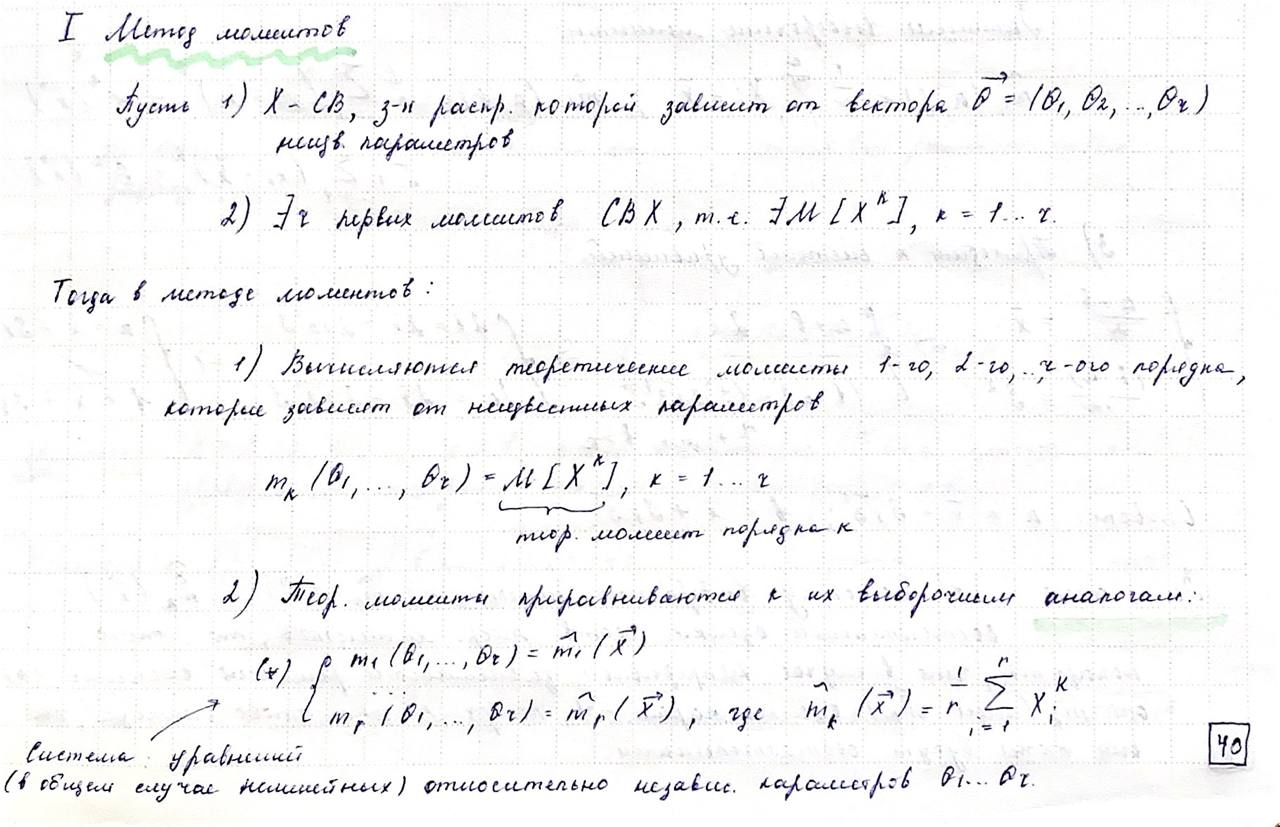
\includegraphics[scale=0.4]{pics/17_1.jpg}}
	\end{figure}
	\clearpage
	\begin{figure}[!h]
		\center{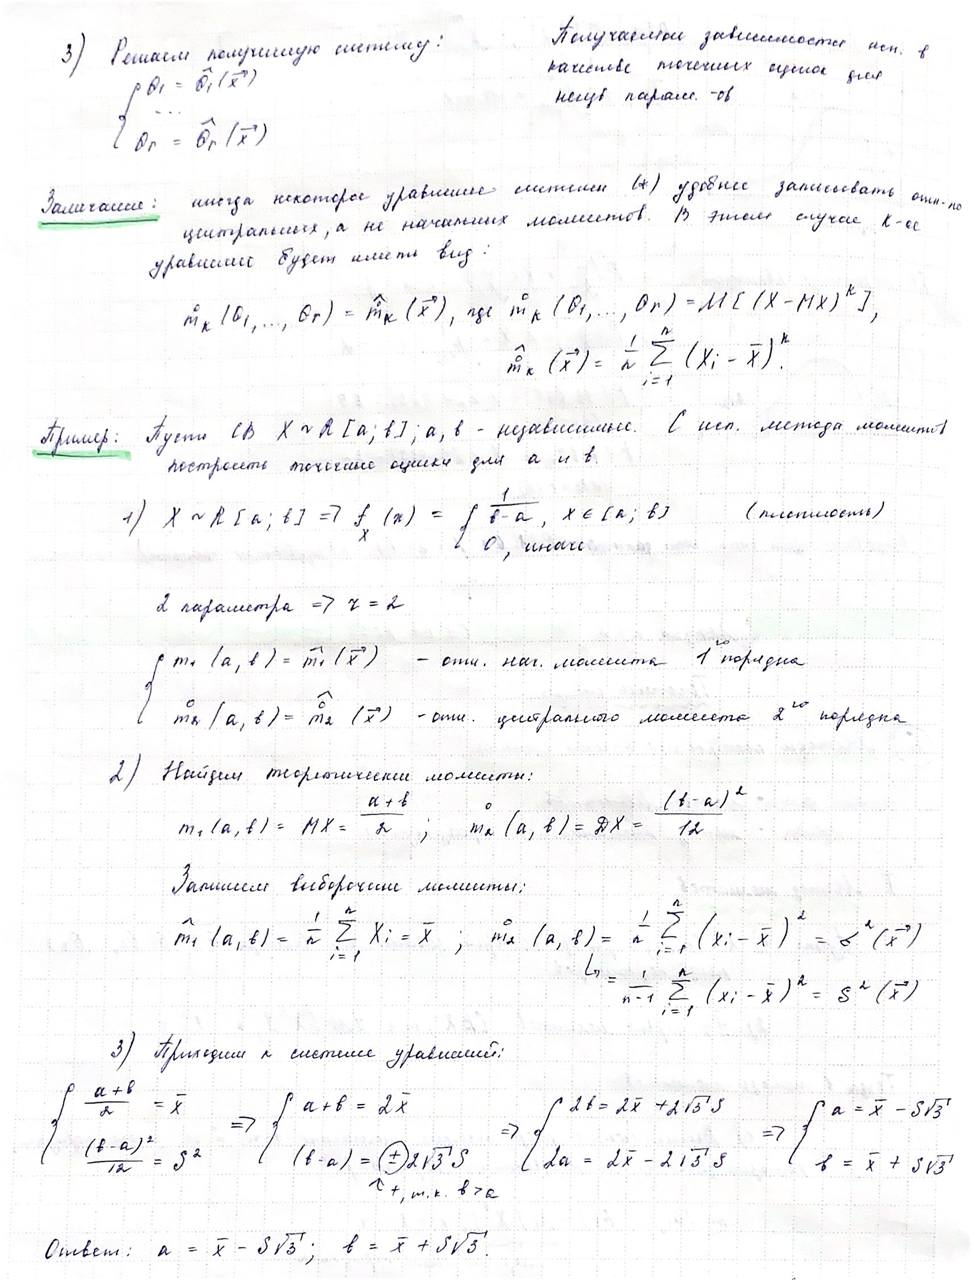
\includegraphics[scale=0.51]{pics/17_2.jpg}}
	\end{figure}
	
	\item \textbf{Постановка задачи идентификации неизвестных параметров закона распределения случайной величины. Определение точечной оценки. Описать метод максимального правдоподобия
		построения точечной оценки. Привести пример.}
	
	Ответ на первый и второй вопрос смотреть в ответах на вопрос 11.
	
	\begin{figure}[!h]
		\center{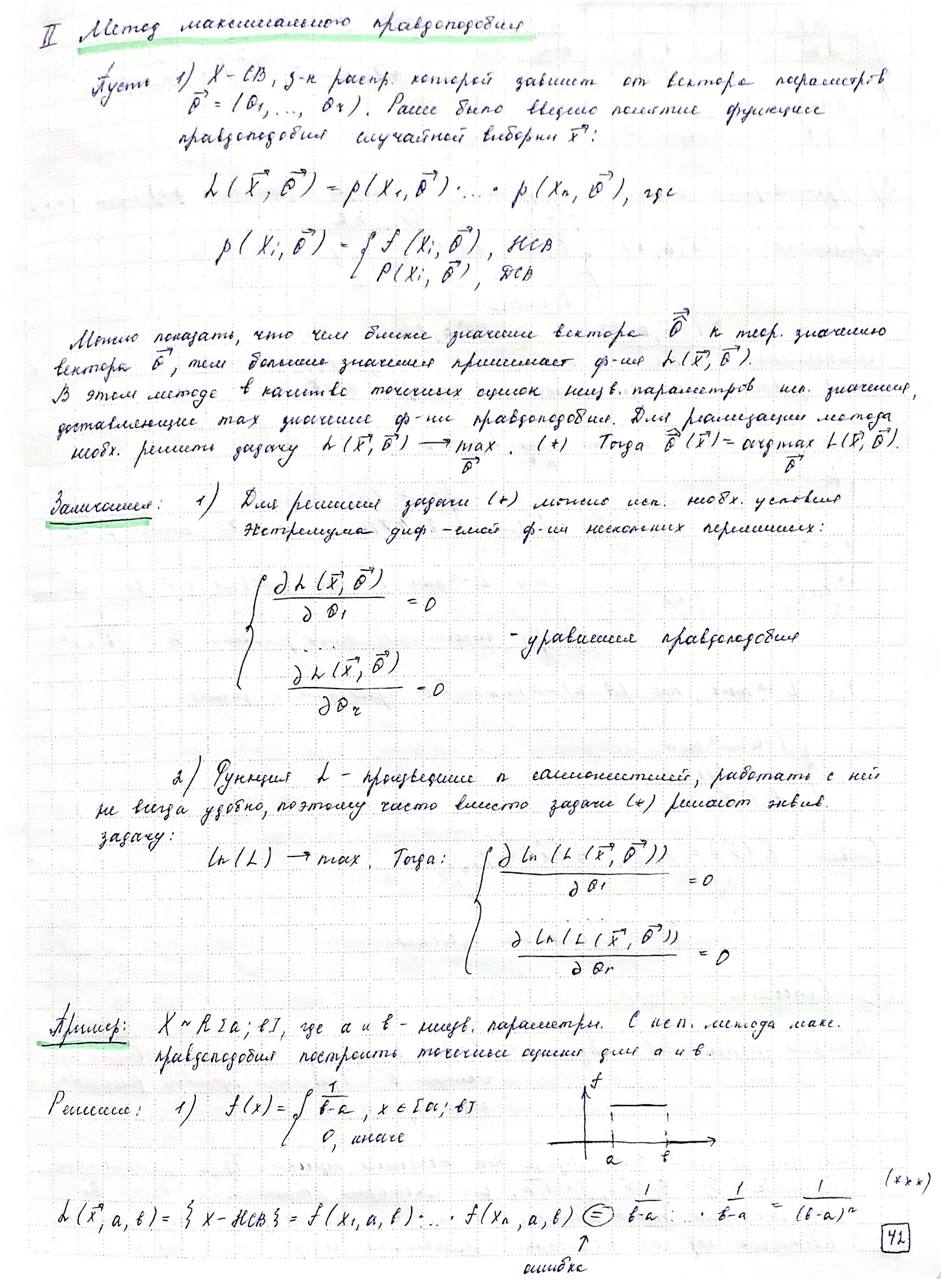
\includegraphics[scale=0.45]{pics/18_1.jpg}}
	\end{figure}
	%\clearpage
	\begin{figure}[!h]
		\center{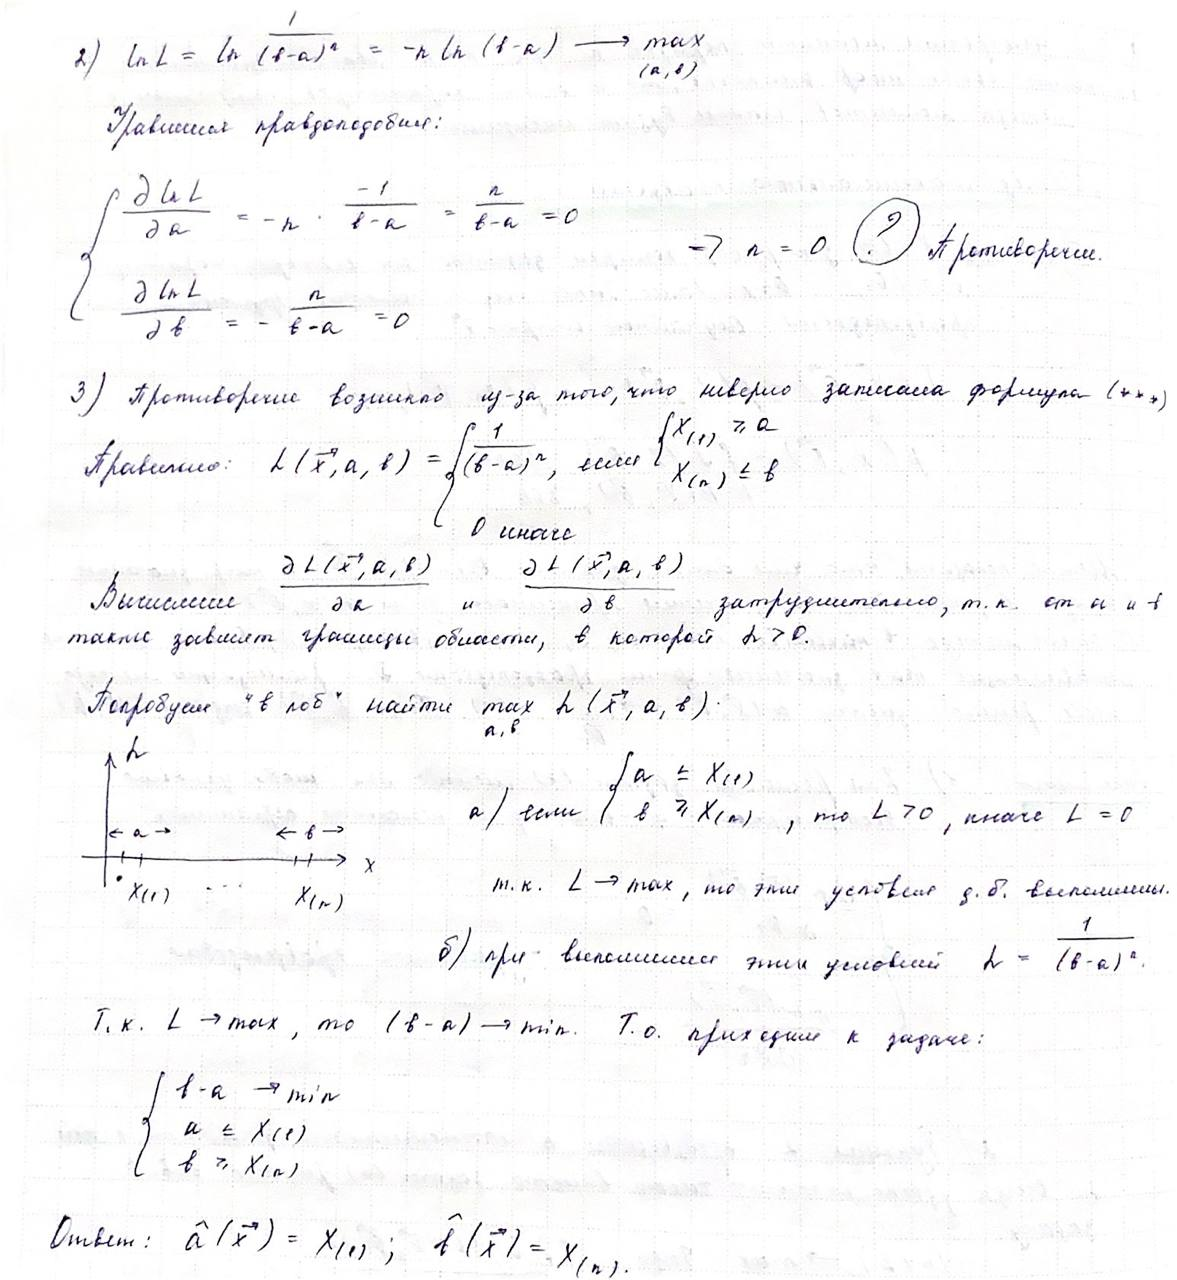
\includegraphics[scale=0.45]{pics/18_2.jpg}}
	\end{figure}

	\clearpage
	
	\item \textbf{Постановка задачи идентификации неизвестных параметров закона распределения случайной величины. Сформулировать определение $\gamma$-доверительного интервала. Сформулировать
		определение центральной статистики и изложить общий алгоритм построения $\gamma$-доверительного интервала для скалярного параметра.}
	
	Ответ на первый вопрос смотреть в ответах на вопрос 11.
	
	\begin{figure}[!h]
		\center{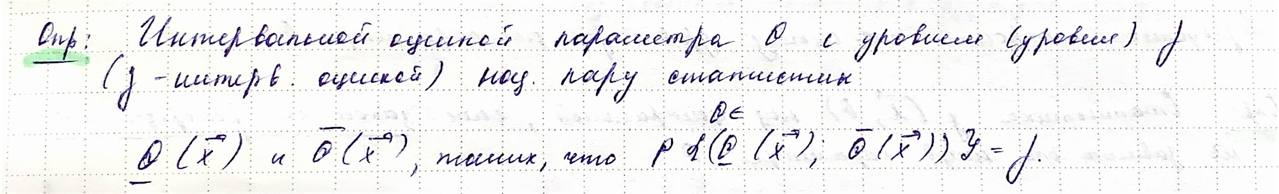
\includegraphics[scale=0.42]{pics/19_1.jpg}}
	\end{figure}
	%\clearpage
	\begin{figure}[!h]
		\center{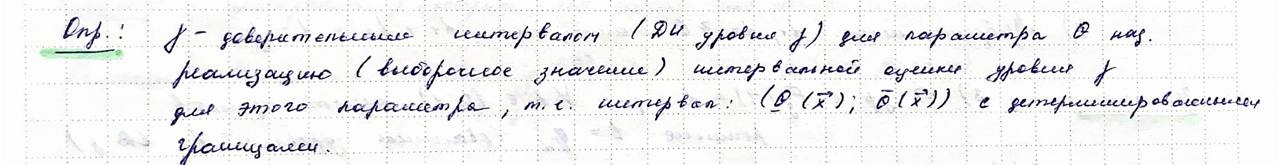
\includegraphics[scale=0.42]{pics/19_2.jpg}}
	\end{figure}
	\begin{figure}[!h]
		\center{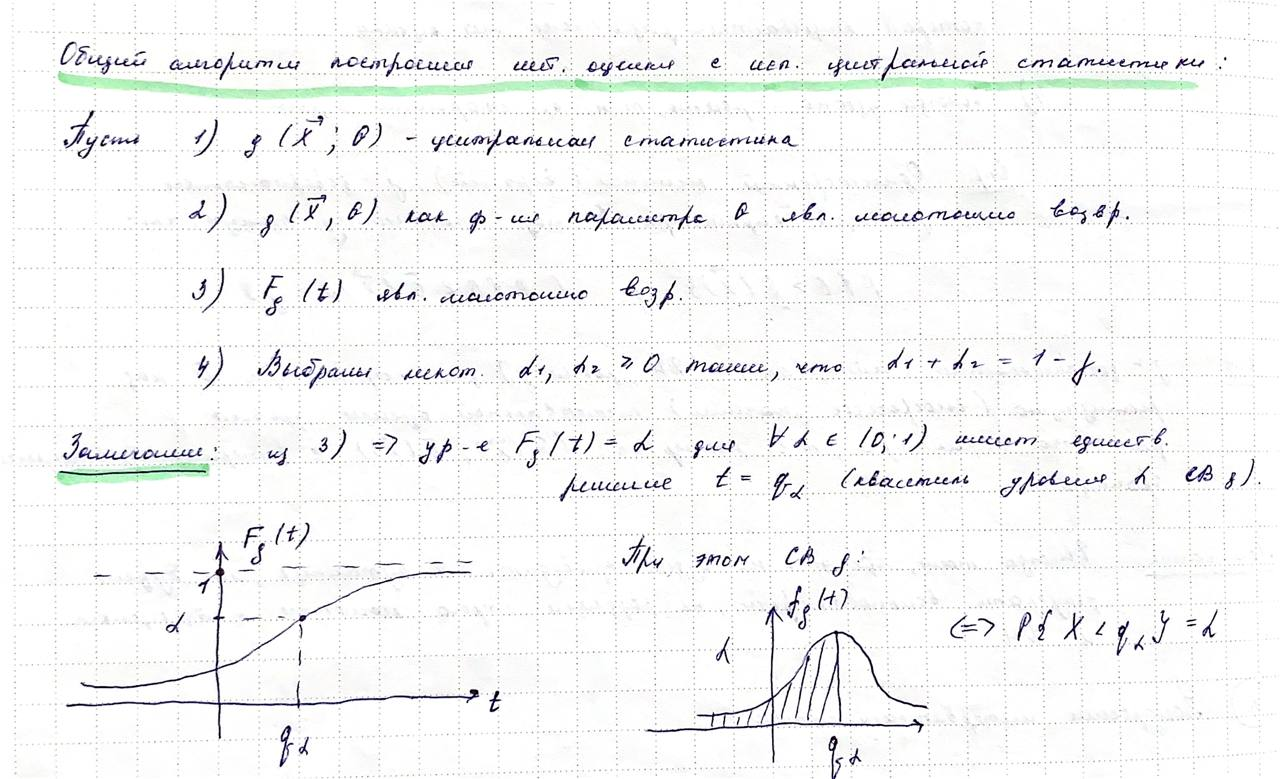
\includegraphics[scale=0.42]{pics/19_3.jpg}}
	\end{figure}
	\clearpage
	\begin{figure}[!h]
		\center{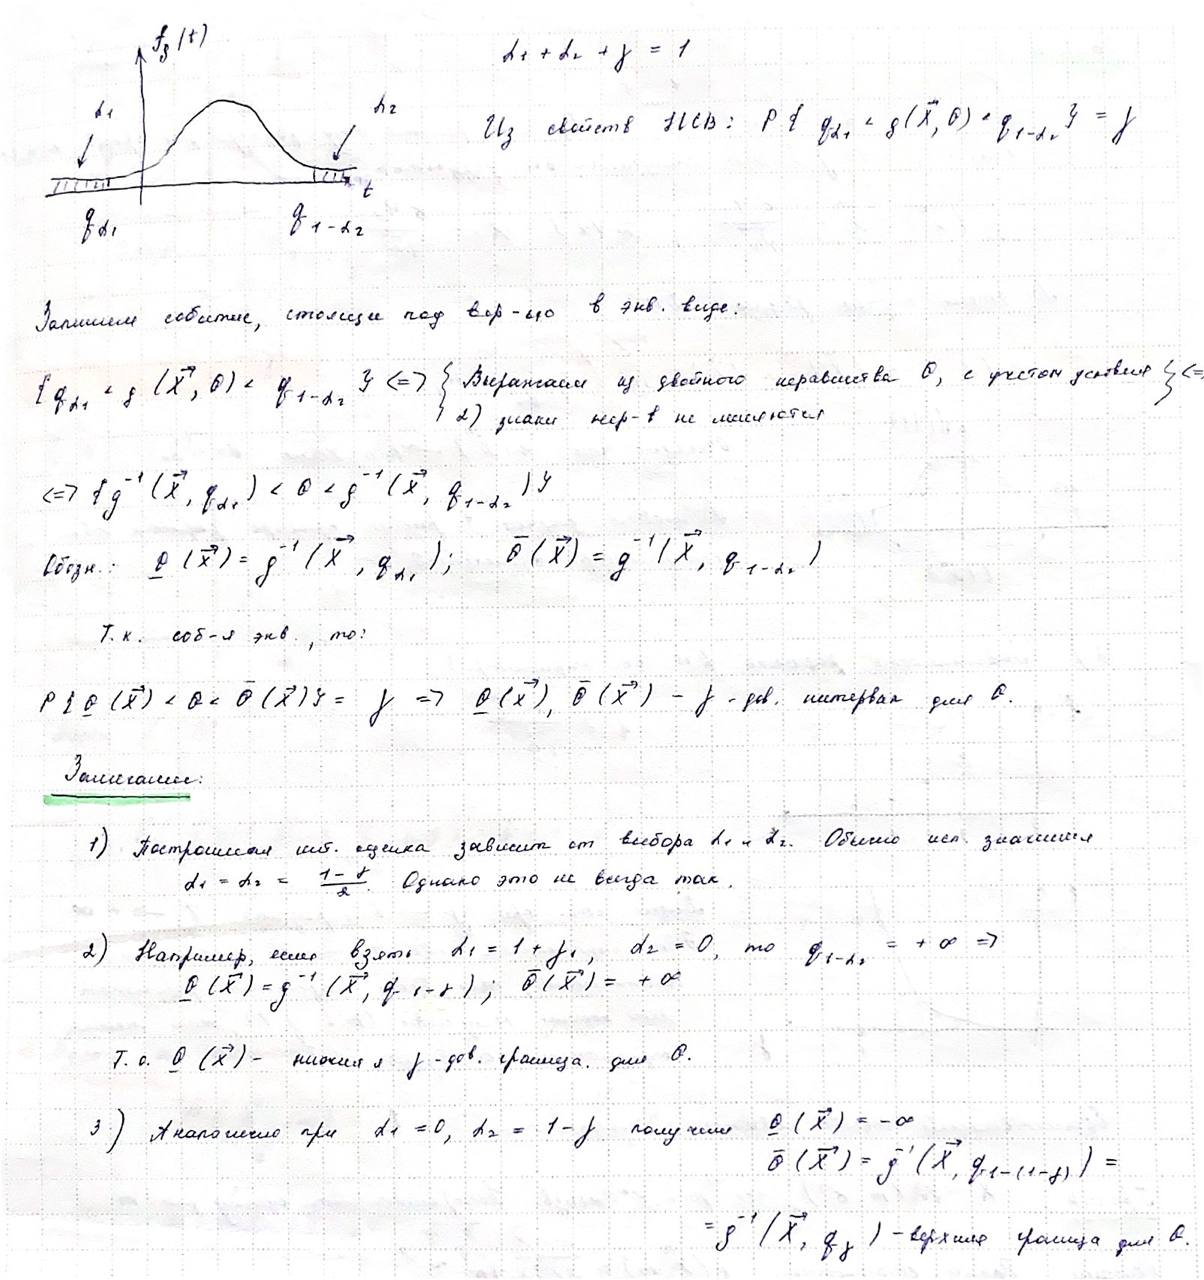
\includegraphics[scale=0.42]{pics/19_4.jpg}}
	\end{figure}

	\clearpage
	
	\item \textbf{Постановка задачи идентификации неизвестных параметров закона распределения случайной величины. Сформулировать определение $\gamma$-доверительного интервала. Сформулировать
		определение центральной статистики. Изложить и обосновать метод построения доверительного интервала для математического ожидания нормальной случайной величины в случае
		известной дисперсии}
	
	Ответ на первый вопрос смотреть в ответах на вопрос 11.
	
	Ответ на второй и третий вопрос смотреть в ответах на вопрос 19.
	
	\begin{figure}[!h]
		\center{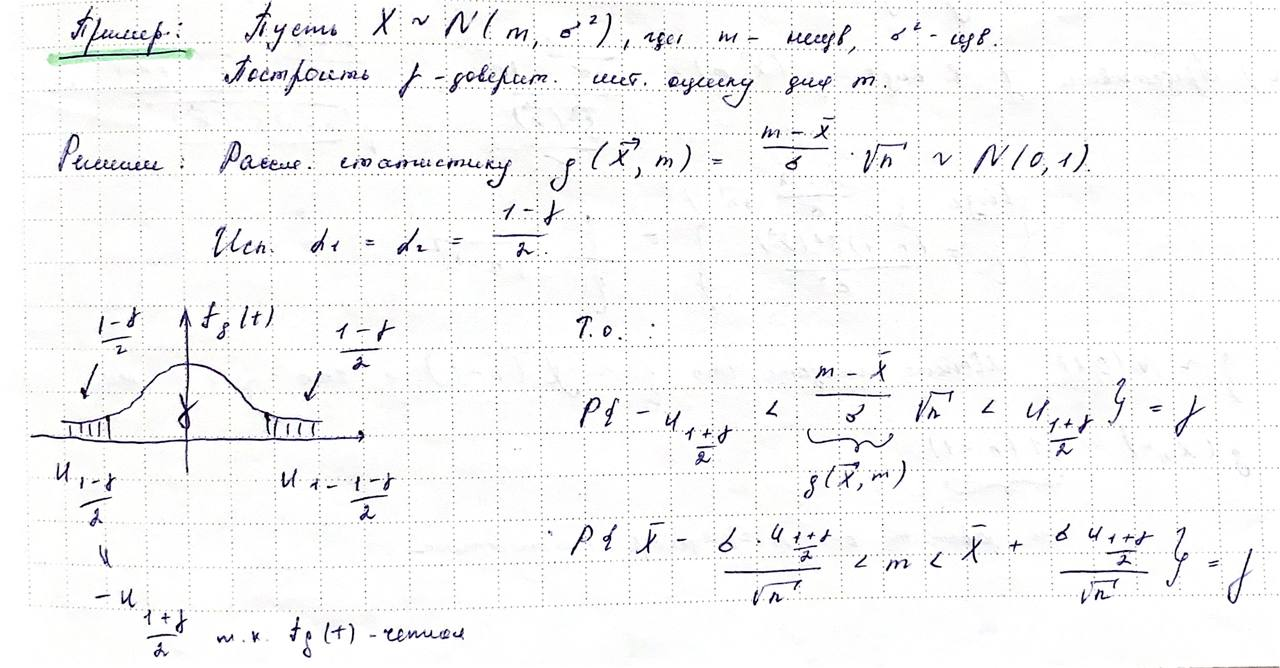
\includegraphics[scale=0.4]{pics/20.jpg}}
	\end{figure}
	
	\clearpage
	
	\item \textbf{Постановка задачи идентификации неизвестных параметров закона распределения случайной величины. Сформулировать определение $\gamma$-доверительного интервала. Сформулировать
		определение центральной статистики. Изложить и обосновать метод построения доверительного интервала для математического ожидания нормальной случайной величины в случае
		неизвестной дисперсии}
	
	Ответ на первый вопрос смотреть в ответах на вопрос 11.
	
	Ответ на второй и третий вопрос смотреть в ответах на вопрос 19.
	
	\begin{figure}[!h]
		\center{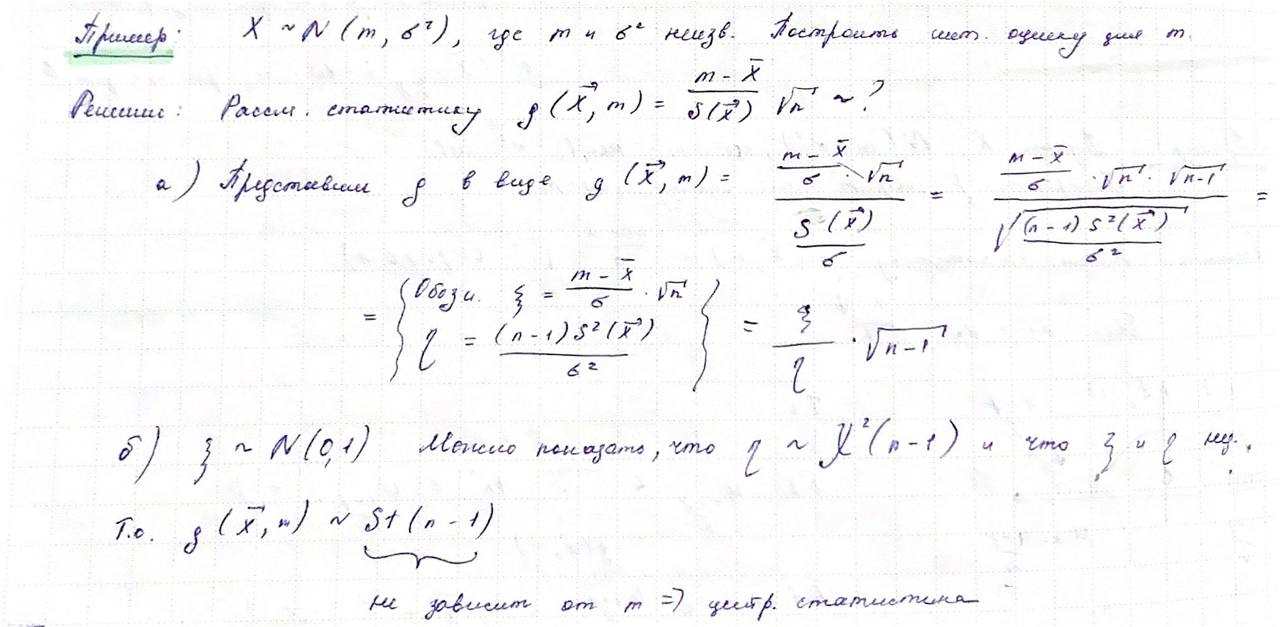
\includegraphics[scale=0.4]{pics/21_1.jpg}}
	\end{figure}
	\begin{figure}[!h]
		\center{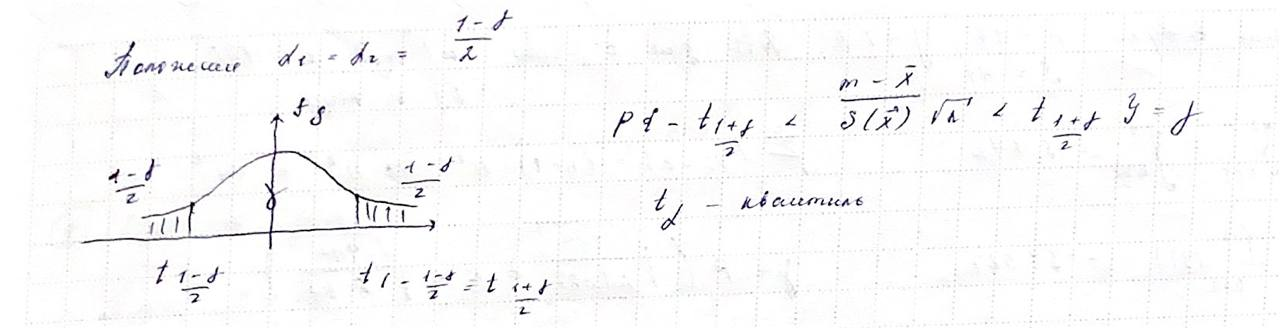
\includegraphics[scale=0.4]{pics/21_2.jpg}}
	\end{figure}

	\clearpage
	
	\item \textbf{Постановка задачи идентификации неизвестных параметров закона распределения случайной величины. Сформулировать определение $\gamma$-доверительного интервала. Сформулировать
		определение центральной статистики. Изложить и обосновать метод построения доверительного интервала для дисперсии нормальной случайной величины.}
	
	Ответ на первый вопрос смотреть в ответах на вопрос 11.
	
	Ответ на второй и третий вопрос смотреть в ответах на вопрос 19.
	
	\begin{figure}[!h]
		\center{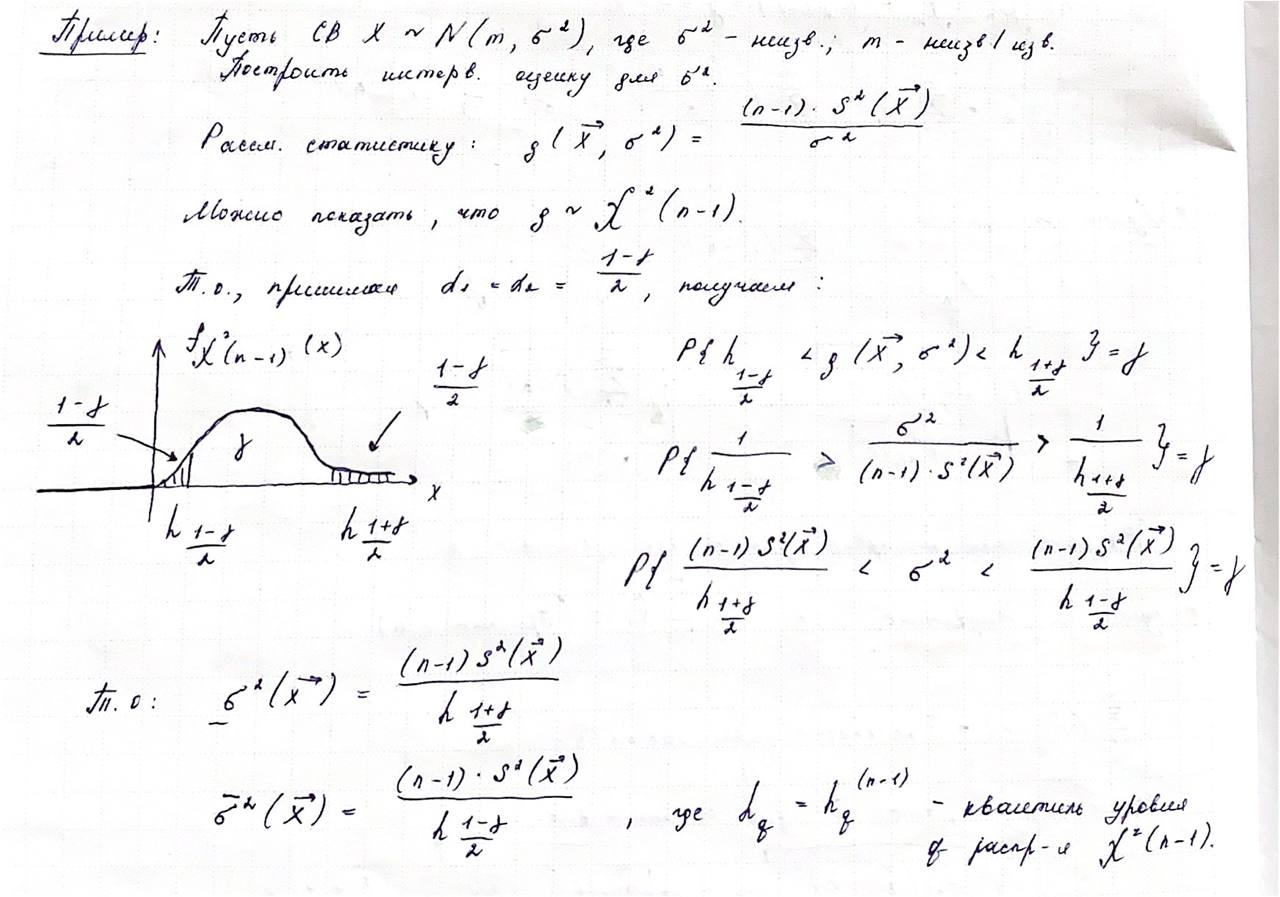
\includegraphics[scale=0.4]{pics/22.jpg}}
	\end{figure}
	
\end{enumerate}

\end{document}